\documentclass[
    12pt
    ,oneside
    ,a4paper
    ,chapter=TITLE
    ,section=TITLE
    ,sumario=abnt-6027-2012]{abntex2}
 
\usepackage{packages/abnt-UTP}
\usepackage{graphicx}
\usepackage{placeins}
\usepackage{xspace}
 
% =================================================================================================
% INFORMAÇÕES GERAIS
% =================================================================================================
 
\titulo{Desenvolvimento de um Compilador e Interpretador Didático Nativo para Dispositivos Móveis Voltado ao Aprendizado de Lógica de Programação}
 
\autor{Vinicius Rodrigues da Costa}
 
\orientador{Prof. Diogenes Cogo Furlan}
 
\preambulo{Trabalho de Conclusão de Curso apresentado ao curso de Bacharelado em Ciência da
Computação da Faculdade de Ciências Exatas e de Tecnologia da Universidade Tuiuti do Paraná,
como requisito à obtenção do grau de Bacharel.}
 
\instituicao{Universidade Tuiuti do Paraná}
\local{Curitiba}
\data{\the\year}

% Citações ajustadas à NBR 10520:2023: sobrenomes com apenas a inicial maiúscula
% e uso de \textit{et al.} somente para obras com quatro ou mais autores.
\newcommand{\citeAho}{(Aho \textit{et al.}, 2007)}
\newcommand{\citeAhoNoschang}{(Aho \textit{et al.}, 2007; Noschang \textit{et al.}, 2014)}
\newcommand{\citeAlgaraibeh}{(Algaraibeh; Dousay; Jeffery, 2020)}
\newcommand{\citeCoelho}{(Coelho; Marques; Oliveira, 2023)}
\newcommand{\citeDimp}{(De Silva \textit{et al.}, 2013)}
\newcommand{\citeFgv}{(Meirelles, 2025)}
\newcommand{\citeIbge}{(IBGE, 2024)}
\newcommand{\citeLiang}{(Liang; Li; Chen, 2014)}
\newcommand{\citeMarceau}{(Marceau; Fisler; Krishnamurthi, 2011)}
\newcommand{\citeNeri}{(Neri; Dias; Gurjão, 2025)}
\newcommand{\citeNoschang}{(Noschang \textit{et al.}, 2014)}
\newcommand{\citeOloo}{(Oloo; Robert, 2020)}
\newcommand{\citeSlany}{(Slany, 2014)}
\newcommand{\citeTims}{(Tims \textit{et al.}, 2024)}

\newcommand{\textAho}{Aho \textit{et al.} (2007)\xspace}
\newcommand{\textAlgaraibeh}{Algaraibeh, Dousay e Jeffery (2020)\xspace}
\newcommand{\textDimp}{De Silva \textit{et al.} (2013)\xspace}
\newcommand{\textLiang}{Liang, Li e Chen (2014)\xspace}
\newcommand{\textMarceau}{Marceau, Fisler e Krishnamurthi (2011)\xspace}
\newcommand{\textNeri}{Neri, Dias e Gurjão (2025)\xspace}
\newcommand{\textNoschang}{Noschang \textit{et al.} (2014)\xspace}
\newcommand{\textOloo}{Oloo e Robert (2020)\xspace}
\newcommand{\textSlany}{Slany (2014)\xspace}
\newcommand{\textSweller}{Sweller (1988)\xspace}
\newcommand{\citeCarga}{(Sweller; van Merriënboer; Paas, 1998)}

% Mantém os títulos das ilustrações em letras maiúsculas tanto no corpo do
% trabalho quanto nas respectivas listas.
\renewcommand{\legenda}[2][]{%
    \centering
    \caption[\MakeTextUppercase{#2}]{\maybeLabel{#1}\MakeTextUppercase{#2}}%
}
 
% =================================================================================================
\begin{document}
% =================================================================================================

% O espaçamento global é definido no início do documento pelo gabarito da UTP.
% Os elementos com espaçamento específico continuam controlados localmente.
 
% -------------------------------------------------------------------------------------------------
% ELEMENTOS PRÉ-TEXTUAIS
% -------------------------------------------------------------------------------------------------
 
\imprimircapa
\imprimirfolhaderosto
 
% -------------------------------------------------------------------------------------------------
% RESUMO
% -------------------------------------------------------------------------------------------------
\begin{resumo}

Este trabalho apresenta o desenvolvimento do Luminthor, um Ambiente Integrado de
Desenvolvimento (IDE) textual para apoio ao ensino de lógica de programação em dispositivos
móveis. O objetivo é integrar escrita, análise, execução e depuração de programas didáticos
no próprio dispositivo. A metodologia caracteriza-se como pesquisa aplicada articulada ao
desenvolvimento experimental de \textit{software}, com especificação da linguagem Lumi,
motor de compilação e interpretação em Rust e interface Flutter integrada por FFI. O
protótipo oferece editor com autocompletar, arquivos locais, trilha com seis módulos e
18 aulas, visualização de tokens e Árvore Sintática Abstrata (AST), diagnósticos em
português e depurador por rastro de execução. A verificação técnica documentada aprovou
65 testes Rust e 155 testes Flutter. A avaliação por formulário reuniu 12 envios, dos
quais uma recusa foi excluída. Entre os 11 respondentes consentidos, oito declararam
instalar e abrir o aplicativo e responderam aos oito itens de usabilidade. As medianas
variaram de 4,5 a 5,0 em uma escala de cinco pontos, com concordância entre 75,0\% e
100\% por item. Os comentários apontaram dificuldades de navegação, identificação do
depurador, digitação e interpretação de um diagnóstico. Os registros das três tarefas
práticas apresentaram informações compatíveis com resultados esperados, mas foram
incompletos para confirmar todos os procedimentos solicitados. Os achados indicam
percepção favorável entre os usuários que experimentaram o aplicativo, com limites
associados à amostra reduzida, à predominância de experiência prévia e ao autorrelato.
A contribuição é a integração de processamento local e recursos didáticos em um único
ambiente móvel; ganho de aprendizagem e desempenho em dispositivos exigem avaliação
específica. A validação é, portanto, parcial: os recursos implementados e a aceitação
declarada não comprovam os benefícios pedagógicos esperados para iniciantes.
 
    \palavraschave{Ensino de programação; Compiladores didáticos; Dispositivos móveis; Ambientes
    de desenvolvimento; Lógica de programação}
\end{resumo}
 
% -------------------------------------------------------------------------------------------------
% LISTAS
% -------------------------------------------------------------------------------------------------
\listadecodigos
\listadefiguras
\listadegraficos
\listadequadros
 
% -------------------------------------------------------------------------------------------------
% SIGLAS
% -------------------------------------------------------------------------------------------------
\begin{siglas}
    \item[ABNT]   Associação Brasileira de Normas Técnicas
    \item[ACM]    \textit{Association for Computing Machinery} (Associação para Computação)
    \item[AOT]    \textit{Ahead-Of-Time} (Compilação Antecipada)
    \item[API]    \textit{Application Programming Interface} (Interface de Programação de Aplicações)
    \item[ARM]    \textit{Advanced RISC Machine} (Máquina Avançada de Conjunto Reduzido de Instruções)
    \item[AST]    \textit{Abstract Syntax Tree} (Árvore Sintática Abstrata)
    \item[BNF]    \textit{Backus-Naur Form} (Forma de Backus-Naur)
    \item[DIMP]   \textit{Distributed Integrated Development Environment for Mobile Platforms} (Ambiente Integrado de Desenvolvimento Distribuído para Plataformas Móveis)
    \item[EBNF]   \textit{Extended Backus-Naur Form} (Forma Estendida de Backus-Naur)
    \item[FFI]    \textit{Foreign Function Interface} (Interface de Funções Externas)
    \item[FGV]    Fundação Getulio Vargas
    \item[FGVcia] Centro de Tecnologia de Informação Aplicada da Fundação Getulio Vargas
    \item[GB]     \textit{Gigabyte} (Unidade de medida de informação digital)
    \item[GLC]    Gramática Livre de Contexto
    \item[IBGE]   Instituto Brasileiro de Geografia e Estatística
    \item[ILDE]   \textit{Integrated Learning Development Environment} (Ambiente Integrado de Desenvolvimento para Aprendizagem)
    \item[IDE]    \textit{Integrated Development Environment} (Ambiente Integrado de Desenvolvimento)
    \item[iOS]    \textit{iPhone Operating System} (Sistema Operacional do iPhone)
    \item[JIT]    \textit{Just-In-Time} (Compilação em Tempo de Execução)
    \item[JVM]    \textit{Java Virtual Machine} (Máquina Virtual Java)
    \item[LLVM]   \textit{Low Level Virtual Machine} (Máquina Virtual de Baixo Nível)
    \item[MIT]    \textit{Massachusetts Institute of Technology} (Instituto de Tecnologia de Massachusetts)
    \item[MVVM]   \textit{Model-View-ViewModel} (Modelo, Visão e Modelo de Apresentação)
    \item[POO]    Programação Orientada a Objetos
    \item[PNAD]   Pesquisa Nacional por Amostra de Domicílios
    \item[R\&D]   \textit{Research and Development} (Pesquisa e Desenvolvimento)
    \item[RAM]    \textit{Random Access Memory} (Memória de Acesso Aleatório)
    \item[RISC]   \textit{Reduced Instruction Set Computer} (Computador com Conjunto Reduzido de Instruções)
    \item[SDK]    \textit{Software Development Kit} (Kit de Desenvolvimento de Software)
    \item[TCC]    Trabalho de Conclusão de Curso
    \item[UI]     \textit{User Interface} (Interface do Usuário)
    \item[UX]     \textit{User Experience} (Experiência do Usuário)
    \item[VS Code] \textit{Visual Studio Code} (Editor de código da Microsoft)
\end{siglas}
 
% -------------------------------------------------------------------------------------------------
% SÍMBOLOS
% -------------------------------------------------------------------------------------------------
\begin{simbolos}
    \item[$ \Sigma $]             Somatório
    \item[$ \prod $]              Produtório
    \item[$ \in $]                Pertence
    \item[$ \notin $]             Não pertence
    \item[$ \mathcal{O}(n) $]     Notação Big O
    \item[$ \forall $]            Para todo (quantificador universal)
    \item[$ \exists $]            Existe (quantificador existencial)
    \item[$ \rightarrow $]        Produção gramatical
    \item[$ \epsilon $]           Palavra vazia (cadeia nula)
    \item[$ \mid $]               Alternativa em regra de produção
\end{simbolos}
 
\sumario
 
% =================================================================================================
% ELEMENTOS TEXTUAIS
% =================================================================================================
\textual
 
% =================================================================================================
% CAPÍTULO 1 — INTRODUÇÃO
% =================================================================================================
\chapter{Introdução}
\label{cap:introducao}
 
A aprendizagem de lógica de programação é frequentemente apontada como um dos maiores desafios
nos cursos de Ciência da Computação ao redor do mundo. Estudos demográficos conduzidos pela
\textit{Association for Computing Machinery} (ACM) demonstram que as taxas de reprovação e evasão
nas disciplinas introdutórias de computação persistem em patamares preocupantes, evidenciando
que o problema não é localizado, mas sistêmico \citeTims. No Brasil, esse quadro é
agravado por uma dupla ordem de desafios: as barreiras pedagógicas associadas ao uso de
determinadas ferramentas de desenvolvimento utilizadas no ensino e as barreiras socioeconômicas
que limitam o acesso à infraestrutura computacional.
 
No que diz respeito às barreiras pedagógicas, o uso de Ambientes Integrados de Desenvolvimento
(IDEs) profissionais em disciplinas introdutórias constitui um dos principais fatores
desfavoráveis. Essas ferramentas foram concebidas com foco na produtividade da indústria de
software, não no processo de ensino. Consequentemente, expõem o aprendiz a um excesso de
configurações avançadas, jargões técnicos e, em muitos casos, à barreira do idioma inglês nas
interfaces e mensagens de erro \citeNoschang. Como resultado direto, o estudante iniciante
vê-se forçado a gerenciar uma elevada carga cognitiva, desviando sua atenção da lógica fundamental
da programação para tentar decifrar mensagens de compilação genéricas e pouco elucidativas
\citeMarceau.
 
\begin{figure}[htb]
\centering
\legenda[fig:comparativo-diagnosticos]{Comparação entre diagnóstico técnico e diagnóstico formativo}
\fig{width=\textwidth}{img/comparativo_mensagens_erro.png}
\fonte{O autor.}
\end{figure}

A Figura~\ref{fig:comparativo-diagnosticos} ilustra o contraste entre uma mensagem técnica
genérica, comum em ambientes profissionais, e uma mensagem formativa voltada ao estudante
iniciante, com indicação de linha, causa provável e sugestão de correção.
 
Além das barreiras pedagógicas, há um desafio socioeconômico relevante relacionado ao acesso
à infraestrutura computacional. Dados da Pesquisa Nacional por Amostra de Domicílios Contínua
(PNAD Contínua), realizada pelo IBGE em 2023, evidenciam que o telefone móvel celular é o
principal equipamento de acesso à internet no Brasil, utilizado por 98,8\% dos usuários,
em contraste com a queda contínua do uso de microcomputadores, presente em apenas 34,2\% da
população \citeIbge. Esse cenário é corroborado por levantamentos da Fundação Getulio
Vargas (FGV), segundo os quais há no país 1,3 \textit{smartphone} por habitante, totalizando
272 milhões de aparelhos em uso \citeFgv. Adicionalmente, a PNAD revela que a ausência
de computadores está intimamente associada à renda, sendo substancialmente menor o rendimento
médio nos domicílios sem esses equipamentos \citeIbge. Dessa forma, muitos estudantes
dependem exclusivamente de seus \textit{smartphones} e carecem de um ambiente adequado e
acessível para a prática de programação.
 
% ====================================================
% SUGESTÃO DE IMAGEM 2:
% Ambiente: Gráfico (ambiente \begin{grafico})
% Tipo: Gráfico de barras ou de linhas temporal
% Conteúdo: Evolução do acesso à internet por tipo de dispositivo no Brasil
%   (celular vs. computador) de 2016 a 2023, com dados da PNAD Contínua.
%   Eixo X: anos; Eixo Y: percentual de usuários.
% Objetivo: Evidenciar o crescimento do celular e queda do computador.
% Como criar: Gráfico gerado no Excel/Python com dados do IBGE (PNAD Contínua
%   2023, Tabela 1.1 ou similar), exportado como imagem de alta resolução.
% Tamanho sugerido: width=0.85\textwidth
% ====================================================
 
Diante desse cenário, o problema de pesquisa que norteia este trabalho pode ser sintetizado
na seguinte questão: como desenvolver uma IDE textual móvel, com compilador didático nativo,
capaz de apoiar estudantes iniciantes no aprendizado de lógica de programação em contextos
de acesso restrito a computadores?
 
Para responder ao problema proposto, o objetivo geral desta pesquisa consiste em
desenvolver um aplicativo móvel autossuficiente que atue, de forma integrada, como uma IDE
e como um motor de compilação e interpretação para o ensino prático de programação. Os
objetivos específicos do trabalho são:
 
\begin{alineas}
    \item Projetar uma interface de edição de código adaptada à ergonomia de telas sensíveis ao toque, contemplando recursos como \textit{highlight} de sintaxe, numeração de linhas, autocompletar, modelos de código e abas de visualização para tokens, AST e rastro de execução;
    \item Especificar formalmente uma gramática livre de contexto para a linguagem algorítmica didática Lumi, com sintaxe reduzida e apoio pedagógico em português na interface;
    \item Construir módulos de análise léxica, sintática e semântica capazes de executar nativamente no dispositivo móvel sem dependência de conectividade de rede;
    \item Gerar diagnósticos formativos a partir da análise da Árvore Sintática Abstrata (AST), com localização da falha e sugestões contextualizadas, incluindo a comparação de nomes semelhantes;
    \item Implementar um depurador visual passo a passo que simule o teste de mesa na tela do celular, exibindo o estado das variáveis a cada instrução executada;
    \item Avaliar, em caráter exploratório, a usabilidade percebida do aplicativo, o uso inicial do depurador e a clareza percebida dos diagnósticos por participantes com diferentes níveis de experiência, com atenção aos iniciantes.
\end{alineas}
 
A metodologia adotada para o alcance desses objetivos caracteriza-se como pesquisa aplicada,
articulada ao desenvolvimento de \textit{software}. Foram definidos
a sintaxe da linguagem Lumi e sua modelagem em AST, implementado o motor nativo em Rust e
integrada a interface Flutter. A execução local segue a abordagem de arquiteturas de
compiladores móveis discutidas por \textLiang. O tratamento de erros é fundamentado
na sequência cognitiva de ler, compreender e formular uma resposta \citeMarceau.
A avaliação exploratória utilizou um formulário eletrônico com questões de perfil,
instalação, três tarefas práticas, oito afirmações de usabilidade e dois comentários
opcionais. Dos 12 envios, um registrou recusa e foi excluído; 11 respostas consentidas
compõem o perfil geral, e oito usuários que relataram abertura do aplicativo compõem
as análises de uso. Foram calculadas frequências, medianas e concordância por item,
com categorização dos comentários e exame dos registros das tarefas. O estudo avalia
percepção e relatos de uso, sem medir ganho de aprendizagem, tempos de execução ou
sucesso sem auxílio verificado por observação direta. Os resultados são apresentados
sem identificação nominal dos participantes. A avaliação observada com foco em iniciantes
e os ensaios controlados em smartphones ainda não foram concluídos; por isso, a validação
do apoio pedagógico e da ergonomia móvel permanece parcial.
 
O presente trabalho está organizado da seguinte forma. O Capítulo~\ref{cap:fundamentacao}
apresenta a fundamentação teórica, abordando os conceitos de ensino de lógica de programação,
construção de compiladores didáticos e \textit{mobile learning}. O
Capítulo~\ref{cap:trabalhos_relacionados} discute os trabalhos relacionados, evidenciando o
estado da arte e contrastando a presente pesquisa com as soluções existentes. O
Capítulo~\ref{cap:metodologia} descreve a metodologia, a arquitetura e a
implementação, incluindo a trilha de aprendizagem, a estratégia de testes e o procedimento
de avaliação. O Capítulo~\ref{cap:resultados} apresenta os resultados técnicos e da
avaliação com participantes, seguidos de discussão e limitações. O
Capítulo~\ref{cap:conclusao} apresenta a conclusão, destacando o estágio atual do
projeto, as etapas pendentes e as contribuições esperadas. Por fim, são apresentadas as
referências utilizadas na pesquisa. O Apêndice~\ref{ape:manual_usuario}
(p.~\pageref{ape:manual_usuario}) contém o manual do usuário, com requisitos, instalação,
arquivos, execução de exemplos, diagnósticos e depuração. O
Apêndice~\ref{ape:manual_tecnico} (p.~\pageref{ape:manual_tecnico}) apresenta o manual
técnico, com preparação das ferramentas, compilação, ponte FFI e comandos de verificação.
 
 
% =================================================================================================
% CAPÍTULO 2 — FUNDAMENTAÇÃO TEÓRICA
% =================================================================================================
\chapter{Fundamentação Teórica}
\label{cap:fundamentacao}
 
Este capítulo estabelece os fundamentos teóricos que embasam a pesquisa. A discussão articula-se
em seis eixos estruturais: o desafio cognitivo no aprendizado de programação; a ascensão do
\textit{mobile learning}; a arquitetura clássica de compiladores; os fundamentos das gramáticas
formais; a engenharia do tratamento de erros pedagógicos; e as abordagens para execução de
código em \textit{smartphones}. Ao final, apresenta-se uma síntese crítica que evidencia a
lacuna científica abordada neste trabalho.
 
% -------------------------------------------------------------------------------------------------
\section{O Desafio Cognitivo e a Evasão no Ensino de Programação}
% -------------------------------------------------------------------------------------------------
 
A aprendizagem de algoritmos e programação constitui o principal fator de reprovação nos anos
iniciais da Ciência da Computação. Relatórios demográficos da ACM evidenciam que a taxa de
retenção em cursos de computação permanece sistematicamente baixa \citeTims. Esse fenômeno
não é trivial: ele resulta de um conjunto de fatores cognitivos, motivacionais e instrumentais
que interagem de maneira complexa no processo de aprendizagem inicial.
 
\subsection{Teoria da Carga Cognitiva e o Ensino de Algoritmos}
 
A Teoria da Carga Cognitiva (\textit{Cognitive Load Theory}) tem como uma de suas
referências a formulação de \textSweller. Nesse estudo, o autor discute a capacidade
limitada de processamento e como o esforço de resolução de problemas pode competir com
os recursos necessários à aquisição de esquemas e à aprendizagem.

Para a discussão das interfaces educacionais, adota-se a formulação clássica de
Sweller, van Merriënboer e Paas (1998), que distingue: (1)~carga intrínseca, relacionada
à complexidade do conteúdo e à interação entre seus elementos; (2)~carga extrínseca,
associada à forma de apresentação e a atividades desnecessárias à aprendizagem; e
(3)~carga germânica, associada ao esforço dedicado à construção de esquemas. Essa
classificação posterior não é atribuída ao artigo de 1988 \citeCarga.

\begin{figure}[htb]
\centering
\legenda[fig:carga-cognitiva-programacao]{Distribuição conceitual da carga cognitiva em ambientes de programação}
\fig{width=\textwidth}{img/carga_cognitiva_programacao.png}
\fonte{O autor, com base em Sweller, van Merriënboer e Paas (1998). Percentuais ilustrativos.}
\end{figure}

A Figura~\ref{fig:carga-cognitiva-programacao} sintetiza essa relação ao representar como
ferramentas inadequadas podem ampliar a carga extrínseca e reduzir o espaço cognitivo dedicado
ao raciocínio algorítmico. Os percentuais são ilustrativos e não constituem uma medição do
protótipo.
 
No contexto do ensino de programação, a carga intrínseca já é naturalmente elevada: o aluno
precisa compreender conceitos abstratos como variáveis, fluxos de controle, recursão e estruturas
de dados de forma simultânea. Quando a esse esforço se soma a carga extrínseca imposta por IDEs
profissionais — configuração de compiladores, gerenciamento de dependências, interpretação de
mensagens de erro em inglês — a memória de trabalho do iniciante satura-se rapidamente, reduzindo
a capacidade germânica de construção de novos esquemas mentais de programação \citeNoschang.
 
\subsection{\textit{Misconceptions} e Erros Conceituais Típicos}
 
Grande parte da dificuldade discente provém de concepções errôneas fundamentais, denominadas
\textit{misconceptions} na literatura de educação em computação. Essas concepções incorretas
surgem quando o aprendiz constrói um modelo mental inadequado das abstrações da linguagem,
frequentemente por falta de \textit{feedback} formativo imediato \citeMarceau.
 
As \textit{misconceptions} mais recorrentes em iniciantes incluem: (a)~acreditar que variáveis
armazenam expressões em vez de valores calculados; (b)~confundir atribuição (\texttt{=}) com
comparação de igualdade (\texttt{==}); (c)~não compreender o escopo de variáveis entre blocos
de código; e (d)~utilizar variáveis antes de serem inicializadas. O uso de variáveis não
inicializadas pode resultar em comportamento indefinido, valores inesperados ou falhas de
execução, dependendo do contexto. Para o iniciante, o problema pedagógico está no fato de a
ferramenta profissional normalmente apresentar o sintoma técnico, e não a causa conceitual do
erro \citeAlgaraibeh.
 
\textMarceau demonstraram empiricamente que a eficácia de
mensagens de erro pode ser medida por uma sequência cognitiva composta de três estágios:
\textit{ler} a mensagem, \textit{entender} o real problema subjacente e \textit{formular} uma
correção. Os autores constataram que estudantes frequentemente estagnam no segundo estágio,
pois as mensagens literais do analisador sintático de compiladores tradicionais mascaram erros
estruturais mais profundos, fornecendo informações sobre o sintoma e não sobre a causa.
 
\begin{figure}[htb]
\centering
\legenda[fig:fluxo-resposta-erro]{Fluxo cognitivo de resposta a uma mensagem de erro}
\fig{width=\textwidth}{img/fluxo_resposta_erro.png}
\fonte{Marceau, Fisler e Krishnamurthi (2011), adaptado pelo autor.}
\end{figure}

A Figura~\ref{fig:fluxo-resposta-erro} apresenta o percurso cognitivo esperado diante de uma
mensagem de erro e destaca o ponto em que diagnósticos genéricos tendem a interromper a
formulação de uma correção consciente.
 
\subsection{Taxas de Reprovação e o Cenário Brasileiro}
 
No cenário global, pesquisas indicam que as taxas de reprovação em disciplinas introdutórias de
programação variam entre 30\% e 50\% em diferentes instituições \citeTims. O contexto
brasileiro apresenta características agravantes: muitos cursos adotam linguagens como C ou Java
diretamente na primeira disciplina, sem uma transição gradual por pseudocódigos ou linguagens
simplificadas, o que intensifica o choque cognitivo inicial do aprendiz.
 
A adoção de ferramentas como o Portugol Studio representa um esforço da comunidade acadêmica
brasileira para mitigar esse problema ao introduzir uma linguagem algorítmica em português, com
mensagens de erro localizadas \citeNoschang. No entanto, essas ferramentas são
primordialmente projetadas para computadores desktop, ignorando a realidade dos estudantes que
dependem exclusivamente de dispositivos móveis.
 
 
% -------------------------------------------------------------------------------------------------
\section{A Barreira Socioeconômica e o \textit{Mobile Learning}}
% -------------------------------------------------------------------------------------------------
 
\subsection{O Contexto de Exclusão Digital no Brasil}
 
A democratização do acesso à educação em computação esbarra em um obstáculo estrutural de
profunda relevância: a desigualdade no acesso a computadores. Dados do Instituto Brasileiro de
Geografia e Estatística (IBGE, 2024) revelam que o telefone celular alcançou a quase
universalidade, sendo utilizado por 98,8\% dos usuários de internet no Brasil. Em contraste, o
acesso por microcomputadores tradicionais caiu para apenas 34,2\% da população \citeIbge.
Esse declínio não é aleatório: a PNAD Contínua demonstra que a posse de computador está
diretamente correlacionada com a renda familiar, sendo que domicílios nas faixas de menor renda
apresentam taxas de posse de computador dramaticamente menores.
 
O levantamento de Meirelles (2025), publicado pelo Centro de Tecnologia de Informação
Aplicada da Fundação Getulio Vargas (FGVcia), corrobora essa transição de paradigma tecnológico. A pesquisa aponta a existência de 1,3 \textit{smartphone} por habitante no Brasil,
totalizando 272 milhões de aparelhos em uso no país \citeFgv. Esse dado é particularmente
significativo quando se considera que muitos desses dispositivos são o único equipamento
computacional disponível em um domicílio.

A posse de \textit{smartphones}, contudo, não comprova por si só a adequação desses aparelhos
para a prática de programação. Programar em um celular envolve restrições específicas: telas
menores reduzem a área simultânea de leitura do código, teclados virtuais dificultam a digitação
de símbolos recorrentes em linguagens textuais, o armazenamento disponível pode limitar a
instalação de ferramentas pesadas, o desempenho do processador e da memória RAM influencia a
fluidez da compilação e a conectividade pode ser instável ou insuficiente para ambientes
dependentes de servidores externos. Além disso, a ergonomia de uso prolongado em telas sensíveis
ao toque exige interfaces mais compactas, comandos de edição simplificados e retorno visual
objetivo. Assim, o argumento deste trabalho não é que todo celular substitui plenamente um
computador, mas que um ambiente didático projetado especificamente para dispositivos móveis pode
reduzir parte dessas barreiras ao oferecer sintaxe controlada, execução local, interface compacta,
persistência automática, diagnósticos formativos e menor dependência de conectividade.

\begin{grafico}[htb]
    \legenda[graf:dispositivos-acesso-2023]{Distribuição dos dispositivos utilizados para acesso à internet no Brasil em 2023}
    \fig{width=0.75\textwidth}{img/grafico1.png}
    \fonte{IBGE, 2024, adaptado pelo autor.}
\end{grafico}
 
\subsection{Fundamentos do \textit{Mobile Learning}}
 
O \textit{Mobile Learning} (m-\textit{learning}) pode ser definido como qualquer forma de
aprendizagem mediada por um dispositivo móvel, caracterizada pela portabilidade, conectividade,
ubiquidade e interatividade \citeCoelho. Diferentemente do \textit{e-learning} tradicional,
que pressupõe o uso de computadores pessoais em locais fixos, o m-\textit{learning} propõe que
a aprendizagem pode favorecer práticas de estudo em diferentes contextos cotidianos, adaptando-se
às condições e ao ritmo do aprendiz.
 
Revisões sistemáticas da literatura demonstram que ferramentas móveis aplicadas ao ensino de
lógica afetam positivamente o engajamento e a motivação dos estudantes \citeCoelho. O
modelo de aprendizagem ubíqua (\textit{ubiquitous learning}), derivado do m-\textit{learning},
propõe ainda que o dispositivo móvel deve suportar a aprendizagem contínua, integrando-se
naturalmente ao cotidiano do aluno. Esse modelo é especialmente relevante no contexto deste
trabalho, pois um estudante sem computador pode ampliar suas oportunidades de prática quando
dispõe de uma ferramenta que funcione no equipamento já presente em sua rotina.
 
\subsection{Iniciativas de Programação Móvel no Brasil}
 
Iniciativas recentes evidenciam o potencial do m-\textit{learning} no ensino de programação no
contexto brasileiro. O aplicativo LogicProg, desenvolvido para o ensino técnico, demonstrou que
o uso de \textit{smartphones} na resolução interativa de algoritmos melhorou significativamente
a compreensão prática dos alunos, que relataram maior motivação para praticar fora do horário
de aula \citeNeri. Contudo, o aplicativo opera com exercícios pré-definidos, sem a
capacidade de compilar e executar código arbitrário escrito pelo usuário. Essa limitação é
exatamente o problema central que o presente trabalho se propõe a resolver.
 
% \begin{figure}[htb]
% \centering
% \legenda[fig:mlearning-Luminthor]{Posicionamento do Luminthor no ecossistema de aprendizagem móvel}
% \fig{width=\textwidth}{img/mlearning_luminthor.png}
% \fonte{Coelho, Marques e Oliveira (2023), adaptado pelo autor.}
% \end{figure}

% A Figura~\ref{fig:mlearning-Luminthor} posiciona o Luminthor no campo da aprendizagem móvel, destacando
% a combinação entre mobilidade, autonomia, funcionamento \textit{off-line} e retorno imediato
% ao estudante.
 
 
% -------------------------------------------------------------------------------------------------
\section{Arquitetura de Compiladores}
% -------------------------------------------------------------------------------------------------
 
A construção de um compilador didático exige a compreensão profunda da teoria dos compiladores,
campo clássico da Ciência da Computação estabelecido a partir das obras pioneiras de
\textAho. Esta seção apresenta os fundamentos teóricos e práticos
das fases de análise que compõem o \textit{front-end} do compilador proposto.
 
\subsection{Visão Geral e Fases de Compilação}
 
Do ponto de vista da Engenharia de \textit{Software}, o projeto clássico de um compilador
divide-se em duas grandes etapas: a fase de análise (\textit{front-end}) e a fase de síntese
(\textit{back-end}). A fase de análise é responsável por ler o código-fonte, verificar sua
conformidade com as regras da linguagem e construir uma representação interna estruturada do
programa. A fase de síntese, por sua vez, transforma essa representação em código executável
ou em outra forma de saída \citeAho.
 
No contexto deste trabalho, a ênfase recai sobre o \textit{front-end} do compilador, uma vez
que é nessa fase que ocorrem a detecção de erros e a geração de mensagens formativas. O
\textit{back-end} corresponde a um interpretador que percorre a AST e executa as instruções
diretamente no dispositivo, sem geração de código intermediário nativo, abordagem adequada
para fins didáticos \citeLiang.
  
\begin{figure}[htb]
\centering
\legenda[fig:arq_compilador]{Modelo conceitual das fases de análise de um compilador didático}
\fig{width=\textwidth}{img/fluxograma.png}
\fonte{Aho \textit{et al.}, 2007, adaptado pelo autor}
\end{figure}

A Figura~\ref{fig:arq_compilador} organiza o fluxo técnico adotado no Luminthor. O código-fonte
inserido pelo estudante é recebido como entrada textual e processado inicialmente pelo
\textit{lexer}, que produz uma sequência de tokens com lexema, tipo, linha e coluna. Em seguida,
o \textit{parser} verifica a estrutura sintática e constrói a Árvore Sintática Abstrata (AST).
A análise semântica percorre essa árvore para validar declarações, mutabilidade,
escopos e chamadas de função. A partir desses dados, o sistema gera mensagens
pedagógicas contextualizadas e, quando não há erros impeditivos, encaminha a AST ao
interpretador e ao depurador visual. Esse encadeamento fundamenta a arquitetura apresentada no
Capítulo~\ref{cap:metodologia}, na qual cada fase do compilador é exposta ao aplicativo móvel
como um artefato observável pelo estudante. Na implementação atual, a análise semântica
consulta as tabelas de símbolos sem produzir uma AST anotada.
 
\subsection{Análise Léxica}
 
A análise léxica constitui a primeira fase do \textit{front-end} do compilador. O componente
responsável por essa fase é denominado analisador léxico (\textit{lexer} ou \textit{scanner}).
Sua função é ler o código-fonte caractere por caractere e agrupar sequências de caracteres em
unidades com significado mínimo, denominadas tokens ou lexemas \citeAho.
 
Um token é representado por um par \texttt{(tipo, valor)}. Por exemplo, no código
\texttt{x = 10 + y}, os tokens produzidos seriam:
\texttt{(IDENTIFICADOR, "x")}, \texttt{(ATRIBUIÇÃO, "=")},
\texttt{(INTEIRO, "10")}, \texttt{(SOMA, "+")}, \texttt{(IDENTIFICADOR, "y")}.
Espaços em branco, comentários e quebras de linha são normalmente descartados pelo
\textit{lexer}, pois não carregam significado semântico para a maioria das linguagens.
 
A especificação dos tokens é feita por meio de expressões regulares. Cada expressão regular
define um padrão que corresponde a uma categoria de token. Para a linguagem Lumi, os tokens
principais incluem palavras reservadas (\texttt{var}, \texttt{const}, \texttt{if},
\texttt{else}, \texttt{while}, \texttt{for}, \texttt{fn}, \texttt{return}, \texttt{print},
\texttt{and}, \texttt{or}, \texttt{not}, \texttt{in}, \texttt{break} e \texttt{continue}),
identificadores, literais numéricos, literais de texto, valores booleanos e \texttt{null},
operadores aritméticos, relacionais e lógicos, além de delimitadores como parênteses, chaves,
vírgulas e ponto e vírgula \citeNoschang.
 
Um analisador léxico didático deve ainda ser capaz de gerar mensagens de erro localizadas
quando encontrar um caractere inválido, em vez de simplesmente abortar a compilação. Por
exemplo, ao encontrar o caractere \texttt{\#} fora de um comentário, o \textit{lexer} deve
informar: \textit{``Caractere '\#' não reconhecido na linha 5, coluna 12. Verifique se
digitou corretamente o operador''}, em vez da mensagem genérica
\textit{``illegal character''}.
 
\subsection{Análise Sintática e Gramáticas Livres de Contexto}
 
A análise sintática — também denominada \textit{parsing} — é a segunda fase do
\textit{front-end}. O analisador sintático (\textit{parser}) recebe o \textit{stream} de
tokens produzido pelo \textit{lexer} e verifica se a sequência de tokens obedece às regras
gramaticais da linguagem. O formalismo utilizado para especificar a sintaxe de linguagens de
programação é a Gramática Livre de Contexto (GLC), também representada na
notação BNF (\textit{Backus-Naur Form}) ou EBNF (\textit{Extended
Backus-Naur Form}) \citeAho.
 
Uma GLC é definida pela quádrupla $ G = (V, \Sigma, P, S) $, onde:
 
\begin{alineas}
    \item $ V $ é o conjunto de variáveis (símbolos não terminais);
    \item $ \Sigma $ é o conjunto de terminais (tokens da linguagem);
    \item $ P $ é o conjunto de regras de produção da forma $ A \rightarrow \alpha $, onde $ A \in V $ e $ \alpha \in (V \cup \Sigma)^* $;
    \item $ S \in V $ é o símbolo inicial da gramática.
\end{alineas}
 
A linguagem Lumi é uma linguagem didática própria, inspirada em construções recorrentes de
disciplinas introdutórias de algoritmos, mas não corresponde a uma cópia direta do Portugol nem
a uma pseudolinguagem informal. A escolha por palavras reservadas curtas e convencionais
(\texttt{if}, \texttt{while}, \texttt{fn}) busca aproximar o estudante de linguagens textuais
modernas, enquanto a interface, os diagnósticos e os exemplos mantêm a mediação pedagógica em
português. A seguir é apresentado um resumo em EBNF da sintaxe aceita pelo protótipo.
A notação \texttt{*} indica repetição e \texttt{?}
indica um elemento opcional:
 
\begin{codigo}[htb]
\legenda[cod:gramatica]{Resumo da gramática EBNF implementada para a linguagem Lumi}
\begin{lstlisting}[language={}]
programa       ::= (';' | declaracao)*
declaracao     ::= decl_variavel | decl_funcao | comando
decl_variavel  ::= ('var' | 'const') identificador ('=' expressao)?
decl_funcao    ::= 'fn' identificador '(' parametros? ')' bloco
parametros     ::= identificador (',' identificador)*
bloco          ::= '{' (';' | declaracao)* '}'
comando        ::= atribuicao | condicional | laco_while | laco_for
                 | saida | retorno | 'break' | 'continue'
                 | bloco | expressao
atribuicao     ::= identificador operador_atr expressao
operador_atr   ::= '=' | '+=' | '-=' | '*=' | '/='
condicional    ::= 'if' expressao bloco ('else' (bloco | condicional))?
laco_while     ::= 'while' expressao bloco
laco_for       ::= 'for' identificador 'in' expressao bloco
saida          ::= 'print' '(' expressao ')'
retorno        ::= 'return' expressao?
argumentos     ::= expressao (',' expressao)*
expressao      ::= logico_ou
logico_ou      ::= logico_e ('or' logico_e)*
logico_e       ::= igualdade ('and' igualdade)*
igualdade      ::= relacional (('==' | '!=') relacional)*
relacional     ::= aditivo (('<' | '<=' | '>' | '>=') aditivo)*
aditivo        ::= multiplicativo (('+' | '-') multiplicativo)*
multiplicativo ::= unario (('*' | '/' | '%') unario)*
unario         ::= ('not' | '-') unario | primario
primario       ::= numero | texto | 'true' | 'false' | 'null'
                 | identificador | chamada | '(' expressao ')'
chamada        ::= identificador '(' argumentos? ')'
\end{lstlisting}
\fonteautor
\end{codigo}

O ponto e vírgula é aceito como separador opcional; as quebras de linha não são tokens de
controle sintático. Para um \texttt{return} sem expressão, usa-se o fim do bloco ou um
ponto e vírgula para delimitar o comando. As variáveis e os parâmetros não recebem anotações
de tipo: os valores são representados pelo interpretador durante a execução. O comando
\texttt{print} recebe uma expressão, e o protótipo não possui comando de leitura de entrada.
Os operadores lógicos são escritos como \texttt{and}, \texttt{or} e \texttt{not}.
No laço \texttt{for i in N}, a expressão deve produzir um inteiro; a execução percorre os
valores de zero até $N-1$. A sintaxe de intervalo \texttt{0..N} não faz parte do parser atual.
 
A estratégia de \textit{parsing} adotada neste trabalho é a análise descendente recursiva
(\textit{recursive descent parsing}), que é uma abordagem \textit{top-down} especialmente
adequada para implementação manual \citeAho. Nessa estratégia, cada regra de produção
da gramática é mapeada diretamente para um procedimento recursivo no código do \textit{parser}.
A análise descendente recursiva possui vantagens didáticas e práticas: é simples de implementar,
facilita a geração de mensagens de erro contextuais e é suficientemente eficiente para o
tamanho dos programas que um estudante iniciante escreve.
 
\subsection{Árvore Sintática Abstrata (AST)}
 
A Árvore Sintática Abstrata (AST, do inglês \textit{Abstract Syntax Tree}) é a estrutura
central produzida pelo \textit{parser} e utilizada em todas as fases subsequentes do compilador.
Trata-se de uma representação em árvore do código-fonte que captura sua estrutura hierárquica
e seu significado semântico, eliminando detalhes sintáticos irrelevantes como parênteses,
ponto e vírgula e outros delimitadores \citeAho.
 
Na AST, cada nó interno representa um construto da linguagem (um operador, um comando de
controle, uma chamada de procedimento), enquanto as folhas representam os operandos (literais,
identificadores). O percurso (\textit{traversal}) da AST pode ser realizado em diferentes
ordens — pré-ordem, em-ordem e pós-ordem — dependendo da operação desejada.

\begin{figure}[htb]
\centering
\legenda[fig:ast-exemplo]{Representação didática de uma árvore sintática de atribuição}
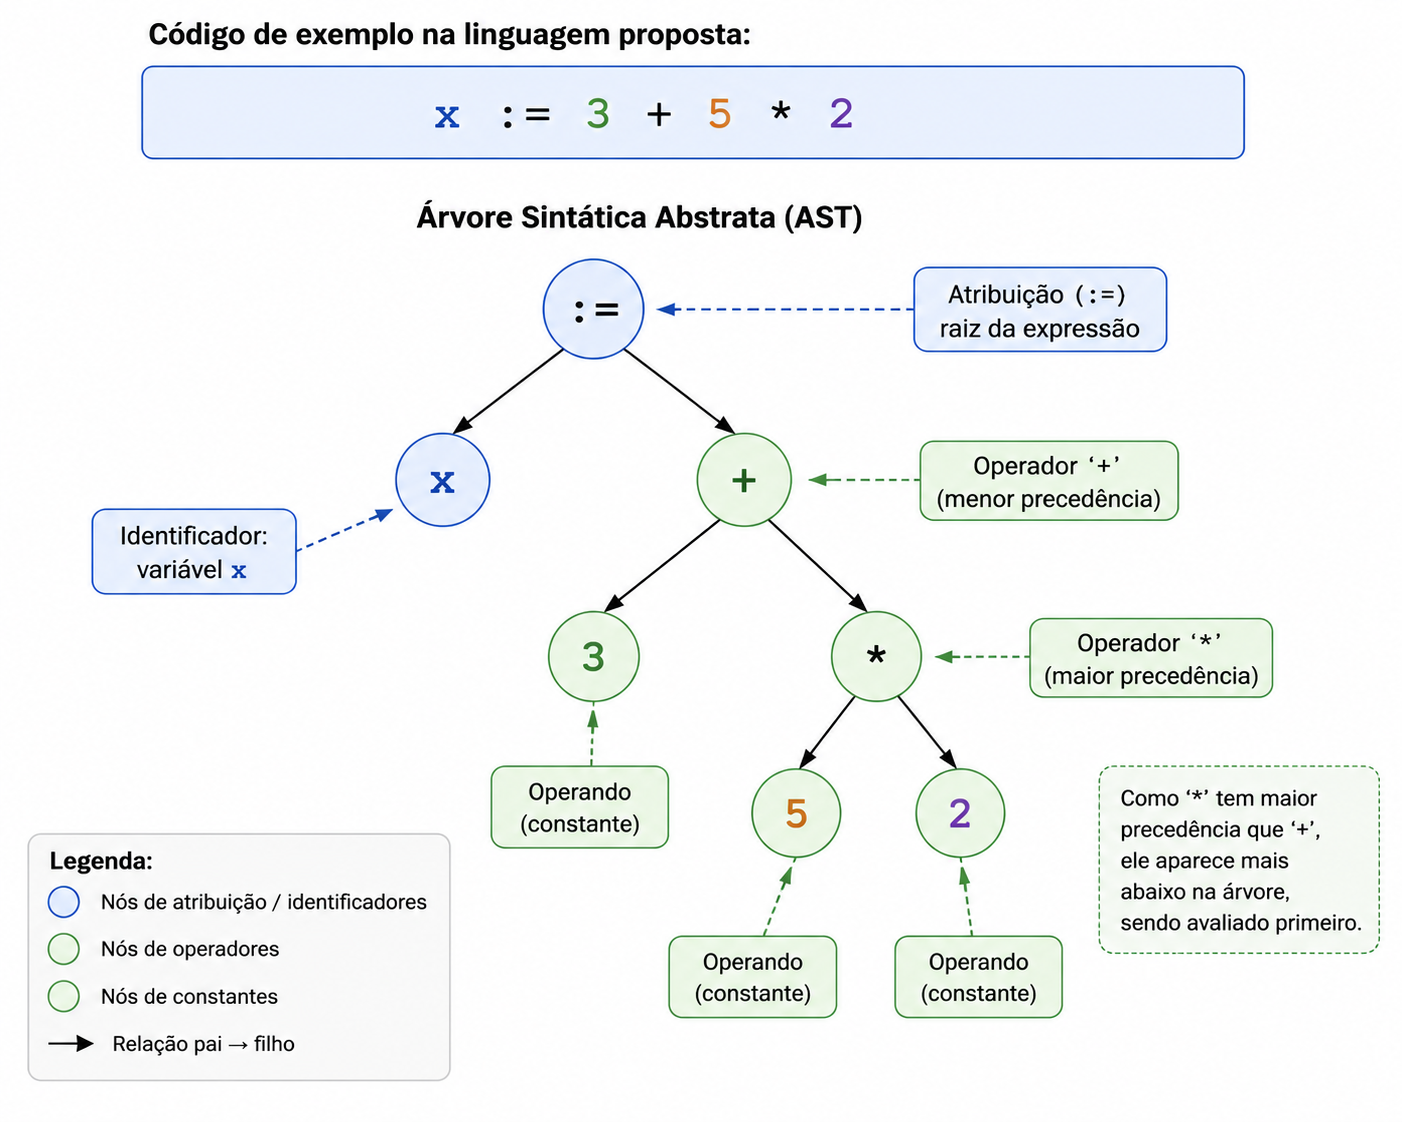
\includegraphics[width=1\textwidth]{img/figuraAST.png}
\fonte{O autor}
\end{figure}
 
% ====================================================
% IMAGEM 8:
% Ambiente: Figura
% Tipo: Diagrama de árvore
% Conteúdo: AST de um exemplo de código simples na linguagem proposta.
%   Por exemplo, o código:
%     x := 3 + 5 * 2
%   deve gerar a AST:
%         :=
%        /  \
%       x    +
%           / \
%          3   *
%             / \
%            5   2
%   Mostrar como a precedência de operadores é capturada na estrutura da árvore.
% Objetivo: Tornar concreto o conceito abstrato de AST para o leitor.
% Como criar: Draw.io, Graphviz (dot language), ou LaTeX/TikZ com \usepackage{forest}.
% Tamanho sugerido: width=0.55\textwidth
% ====================================================


 
A Figura~\ref{fig:ast-exemplo} exemplifica como uma expressão textual é convertida em
estrutura hierárquica. Em uma atribuição como \texttt{x = 3 + 5 * 2}, a multiplicação deve
aparecer em um nível mais profundo da árvore do que a soma, preservando a precedência dos
operadores. A figura usa \texttt{:=} como notação didática de atribuição; na Lumi usa-se
\texttt{=}. Essa representação permite que o estudante visualize por que o compilador interpreta
uma expressão de determinada forma e permite que o sistema relacione erros a nós específicos,
como atribuições, chamadas de função, expressões lógicas ou comandos de repetição.

A inspeção da AST também fornece contexto para os diagnósticos. No protótipo, uma atribuição
armazena o nome de seu destino e a expressão que produzirá o valor. O analisador consulta a
tabela de símbolos para verificar se o nome foi declarado e se pode receber alterações.
Quando encontra um nome desconhecido, procura identificadores semelhantes e apresenta uma
sugestão de correção, quando disponível. Essa associação entre estrutura do programa e
diagnóstico contextual segue o princípio de mensagens voltadas a iniciantes \citeNoschang.
 
\subsection{Análise Semântica e Tabela de Símbolos}
 
A análise semântica é a terceira fase do \textit{front-end} e atua sobre a AST produzida pelo
\textit{parser}. Sua responsabilidade é verificar o \textit{significado} do programa além da
sua estrutura sintática. As verificações semânticas típicas incluem: a declaração de variáveis
antes do uso, a compatibilidade de tipos em expressões e atribuições, a correspondência de
argumentos em chamadas de procedimentos e a detecção de variáveis utilizadas sem inicialização
\citeAho.
 
Uma tabela de símbolos associa identificadores a informações necessárias à análise do
programa. No Luminthor, ela é implementada como uma pilha de tabelas hash. Cada símbolo
registra mutabilidade, indicação de função e quantidade de parâmetros quando aplicável.
O início de um bloco cria uma tabela, e seu encerramento a remove; a busca percorre os escopos
do mais interno ao mais externo. A implementação verifica nomes declarados, atribuição a
constantes, chamadas de função e uso de comandos de controle. A compatibilidade dos valores
usados em operações é verificada durante a interpretação. O protótipo ainda não realiza uma
análise estática geral de tipos ou de inicialização definitiva de variáveis.
 
% ====================================================
% SUGESTÃO DE IMAGEM 9:
% Ambiente: Quadro (ambiente \begin{quadro})
% Tipo: Tabela ilustrativa
% Conteúdo: Exemplo de estado da Tabela de Símbolos durante a execução do
%   analisador semântico de um programa-exemplo. Colunas:
%   Identificador | Tipo | Escopo | Inicializado | Linha de Declaração
%   Linhas com exemplos: x | inteiro | global | sim | 2
%                        nome | texto  | global | não | 3
% Objetivo: Tornar concreto o conceito de tabela de símbolos.
% Tamanho sugerido: width=0.75\textwidth
% ====================================================
 
 
% -------------------------------------------------------------------------------------------------
\section{A Engenharia do Tratamento de Erros Pedagógicos}
% -------------------------------------------------------------------------------------------------
 
\subsection{Taxonomia de Erros em Linguagens de Programação}
 
Os erros em linguagens de programação podem ser classificados segundo o momento em que são
detectados e sua natureza:
 
\begin{alineas}
    \item Erros léxicos: ocorrem durante a análise léxica e envolvem caracteres ou sequências de caracteres não pertencentes ao alfabeto da linguagem. Exemplo: uso do símbolo \texttt{@} fora de um contexto previsto pela gramática;
    \item Erros sintáticos: detectados durante o \textit{parsing}, decorrem da violação das regras gramaticais da linguagem. Exemplo: ausência de fechamento de chaves em uma estrutura condicional;
    \item Erros semânticos: identificados na fase semântica, representam violações de regras de significado. Exemplo: somar uma variável do tipo \texttt{string} com um número sem conversão prevista;
    \item Erros em tempo de execução: manifestam-se durante a interpretação do código. Exemplo: divisão por zero ou limite máximo de passos atingido em um laço.
\end{alineas}
 
Para iniciantes, os erros sintáticos e semânticos são os mais frequentes e os que mais causam
frustração, pois as mensagens geradas por compiladores profissionais geralmente reportam o
sintoma do erro em vez de sua causa pedagógica subjacente \citeMarceau.
 
\subsection{Princípios para Mensagens de Erro Formativas}
 
Com base no estudo de \textMarceau, podem-se definir os
seguintes princípios para o design de mensagens de erro pedagogicamente eficazes:
 
\begin{alineas}
    \item Localização precisa: a mensagem deve indicar com exatidão a linha e coluna onde o erro foi detectado;
    \item Explicação causal: a mensagem deve descrever a \textit{causa} do problema, não apenas o sintoma observado pelo compilador;
    \item Contextualização: a mensagem deve ser redigida considerando o contexto do código circundante, inferindo a intenção provável do aluno;
    \item Sugestão de correção: sempre que possível, a mensagem deve sugerir uma ação corretiva específica e aplicável;
    \item Idioma nativo: mensagens em português eliminam a barreira linguística e permitem que o aluno concentre sua atenção no problema lógico, não na tradução.
\end{alineas}
 
\subsection{O Padrão Visitante (\textit{Visitor Pattern}) na AST}
 
O Padrão de Projeto Visitante (\textit{Visitor Pattern}) permite separar operações de
processamento da estrutura sobre a qual elas atuam. Essa separação orienta a organização dos
percursos da AST, mas o protótipo não implementa uma hierarquia de classes visitantes.
Em Rust, o analisador semântico e o interpretador são módulos próprios que percorrem os tipos
enumerados da AST por correspondência de variantes, utilizando \texttt{match}. O primeiro
registra declarações, verifica escopos e produz diagnósticos; o segundo executa comandos,
atualiza o ambiente e registra passos de execução. Visitantes adicionais para análise estática
de tipos ou de inicialização constituem possibilidades de extensão, e não funcionalidades
implementadas no protótipo \citeAhoNoschang.

Essa separação é particularmente valiosa no contexto didático porque permite acrescentar novas
regras de diagnóstico sem reescrever o \textit{parser} ou alterar a representação central da
AST. Assim, a linguagem pode crescer gradualmente, enquanto os diagnósticos continuam
organizados por responsabilidade técnica e finalidade pedagógica.
 
% ====================================================
% SUGESTÃO DE IMAGEM 10:
% Ambiente: Figura
% Tipo: Diagrama de classes UML simplificado
% Conteúdo: Diagrama UML mostrando a relação entre as classes da AST
%   (NóAST, NóAtribuição, NóSe, NóEnquanto, NóExpressão...)
%   e as classes Visitante (AnalisadorSemântico, GeradorMensagens,
%   InterpretadorExecução). Mostrar as interfaces e a relação de
%   herança/implementação.
% Objetivo: Ilustrar a arquitetura modular do compilador proposto.
% Como criar: Draw.io, StarUML, PlantUML ou similar.
% Tamanho sugerido: width=\textwidth
% ====================================================
 
 
% -------------------------------------------------------------------------------------------------
\section{Viabilidade Técnica: IDEs Móveis e Execução Local}
% -------------------------------------------------------------------------------------------------
 
\subsection{Arquitetura de Plataformas Móveis}
 
O desenvolvimento de um compilador nativo para dispositivos móveis exige a compreensão das
restrições arquiteturais desses sistemas. Os \textit{smartphones} modernos baseados em Android
e iOS operam predominantemente sobre processadores ARM de 64 bits, mas variam amplamente em
memória, armazenamento, qualidade de tela, desempenho térmico e conectividade. Modelos de
entrada frequentemente possuem cerca de 3 GB a 4 GB de RAM, enquanto aparelhos intermediários e
avançados podem alcançar 8 GB, 12 GB ou mais. Para o público-alvo deste trabalho, a referência
prática deve ser o aparelho de entrada: Android 10 ou superior, processador ARM64, pelo menos
3 GB de RAM e aproximadamente 200 MB de armazenamento livre para o aplicativo, exemplos e dados
locais. No iOS, a compatibilidade depende das versões suportadas pelo Flutter e da política de
distribuição da Apple, mas o mesmo princípio de baixo consumo de memória orienta o projeto.
Embora inferiores a computadores desktop, essas especificações são suficientes para executar um
compilador e interpretador de uma linguagem didática, cujos programas tendem a ter poucas
centenas de linhas \citeLiang.

O ecossistema Flutter, adotado como plataforma de desenvolvimento para este projeto, compila o
código Dart para código nativo ARM por compilação AOT (\textit{Ahead-Of-Time}) em versões de
produção, o que favorece desempenho previsível em Android e iOS. Além disso, Flutter oferece
componentes adequados à construção de editor, abas, painéis de diagnóstico e visualizações
interativas, enquanto bibliotecas de persistência local permitem manter código e preferências
sem servidor externo. A principal limitação dessa escolha é o cuidado necessário com consumo de
memória, tamanho do aplicativo e fluidez da interface em telas menores. Por isso, o motor de
compilação é mantido em Rust e integrado por FFI, preservando desempenho, segurança de memória e
portabilidade sem exigir conectividade permanente.
 
\subsection{Abordagens de Execução: Local versus Distribuída}
 
O mercado acadêmico apresenta duas abordagens para IDEs móveis: processamento distribuído
(nuvem) e nativo (local). O sistema DIMP (\textit{Distributed Integrated Development
Environment for Mobile Platforms}) adota o modelo distribuído, delegando a compilação a
servidores externos \citeDimp. Embora esse modelo reduza o consumo computacional local,
sua dependência contínua de conectividade de rede constitui um ponto de falha crítico em
cenários educacionais de vulnerabilidade digital, onde a conexão à internet é instável ou
inexistente.
 
Em contrapartida, projetos como o ambiente Ubi-C demonstraram que o avanço tecnológico já
permite a execução nativa de compiladores em dispositivos móveis. O Ubi-C embutiu os
compiladores Clang e LLVM localmente no Android, possibilitando a interpretação de código
C \textit{off-line} com rastreamento em tempo real e suporte a pontos de parada
(\textit{breakpoints}) \citeLiang. O aplicativo Pocket Code também demonstra a viabilidade
técnica, provando a suficiência de processamento de celulares modernos para IDEs interativas
\citeSlany.
 
% ====================================================
% SUGESTÃO DE IMAGEM 11:
% Ambiente: Quadro (ambiente \begin{quadro})
% Tipo: Tabela comparativa
% Conteúdo: Comparação entre a abordagem distribuída (nuvem) e a abordagem
%   nativa (local) em termos de: dependência de internet, latência de
%   compilação, privacidade do código, consumo de bateria, complexidade de
%   implementação.
% Objetivo: Justificar a escolha da abordagem nativa para o projeto.
% Tamanho sugerido: width=\textwidth
% ====================================================
 
\subsection{Evidências Empíricas sobre Usabilidade Móvel em Programação}
 
Testagens empíricas com compiladores de C/C++ no Android revelam que a mera portabilidade
de uma ferramenta profissional para o celular é insuficiente e gera altas taxas de abandono.
\textOloo constataram que cerca de 67,6\% dos alunos apontaram que lidar com erros e
\textit{bugs} não traduzidos e sem contexto pedagógico foi o maior obstáculo para programar
no celular, superando amplamente as queixas sobre o tamanho reduzido da tela (31,2\%). Esse
dado empírico reforça a premissa central deste trabalho: a interface
gráfica adequada é importante, mas o tratamento pedagógico das mensagens de erro é o
componente mais crítico para a adoção de IDEs móveis no ensino.
 
 
% -------------------------------------------------------------------------------------------------
\section{Síntese da Fundamentação Teórica e Lacuna Científica}
% -------------------------------------------------------------------------------------------------
 
A análise da literatura evidencia que os desafios no ensino de programação não se limitam
à complexidade lógica inerente às linguagens formais. Eles envolvem, de forma interligada,
restrições cognitivas, socioeconômicas e ferramentais. Observa-se que compiladores tradicionais
e IDEs profissionais não foram concebidos com foco pedagógico, resultando em barreiras
adicionais para estudantes iniciantes. A popularização dos \textit{smartphones} e o avanço
das arquiteturas móveis demonstram a viabilidade técnica da execução local de código
diretamente no dispositivo.
 
O Quadro~\ref{quad:comparativo} sumariza como as diferentes ferramentas abordadas na literatura
atendem às necessidades do programador novato, segundo as dimensões mais relevantes identificadas
pela revisão bibliográfica.
 
\begin{quadro}[htb]
\centering
\legenda[quad:comparativo]{Comparação entre ferramentas de compilação e ensino quanto às necessidades do aprendiz}

\resizebox{\textwidth}{!}{
\begin{tabular}{|l|c|c|c|c|c|}
\hline
Ferramenta    & Mobile & Offline & AST para feedback & Mensagens pedagógicas & Português \\
\hline\hline
g++ / Clang   & Não    & Sim    & Sim (interno) & Não    & Não    \\
\hline
Portugol Studio & Parcial & Sim  & Sim (custom.) & Sim    & Sim    \\
\hline
DIMP          & Sim    & Não    & Parcial       & Não    & Não    \\
\hline
Ubi-C         & Sim    & Sim    & Não           & Parcial& Não    \\
\hline
Pocket Code   & Sim    & Sim    & Não           & Parcial& Não    \\
\hline
LogicProg     & Sim    & Sim    & Não           & Sim    & Sim    \\
\hline
Projeto proposto      & Sim    & Sim    & Sim           & Sim    & Sim    \\
\hline
\end{tabular}
}

\vspace{0.2cm}
\fonteautor
\end{quadro}
 
A análise do Quadro~\ref{quad:comparativo} evidencia uma lacuna científica situada na
intersecção entre acessibilidade móvel, execução local e mediação pedagógica. As ferramentas
profissionais oferecem compilação robusta, mas não foram concebidas para reduzir a carga
cognitiva do aprendiz; os ambientes pedagógicos em português contribuem para o ensino inicial,
mas permanecem concentrados no computador; e as soluções móveis existentes tendem a depender de
nuvem, de linguagens profissionais complexas ou de programação por blocos. Assim, ainda carece
de investigação uma IDE textual para \textit{smartphones} que funcione \textit{off-line},
compile ou interprete localmente, apresente linguagem didática em português, trate erros com
explicação semântica e ofereça depuração visual adequada à ergonomia móvel. Essa combinação é
relevante porque ataca simultaneamente a exclusão de acesso ao computador, a dificuldade de
compreender mensagens técnicas e a necessidade de praticar lógica de programação em um ambiente
autossuficiente.
 
O preenchimento desta lacuna fundamenta o propósito do desenvolvimento proposto nos capítulos
a seguir, alinhando rigor arquitetural à inovação no ensino de algoritmos.

% =================================================================================================
% CAPÍTULO 3 — TRABALHOS RELACIONADOS
% =================================================================================================
\chapter{Trabalhos Relacionados}
\label{cap:trabalhos_relacionados}
 
Este capítulo apresenta e analisa criticamente os principais trabalhos da literatura que mais
se aproximam da proposta desta pesquisa. Os trabalhos são discutidos em dois grupos: (1)~IDEs
e compiladores com foco pedagógico para ambientes desktop; e (2)~ferramentas de programação
para dispositivos móveis. Ao final, é apresentada uma análise comparativa que evidencia como
o presente trabalho se distingue e contribui em relação ao estado da arte.
 
 
% -------------------------------------------------------------------------------------------------
\section{IDEs e Compiladores Pedagógicos para Desktop}
% -------------------------------------------------------------------------------------------------
 
\subsection{Portugol Studio}
 
\textNoschang desenvolveram, no Brasil, o Portugol Studio, que é a
referência nacional mais relevante para este trabalho. Trata-se de uma IDE desktop com
linguagem algorítmica em português, analisador sintático com geração de AST e mensagens de
erro formativas localizadas. O sistema implementa um interpretador que percorre a AST gerada
e exibe o estado das variáveis durante a execução, funcionando como um depurador visual básico.
 
As principais contribuições do Portugol Studio para este trabalho são: (a)~a validação do
conceito de linguagem algorítmica em português como facilitadora do aprendizado inicial;
(b)~a demonstração de que mensagens de erro baseadas em análise da AST são pedagogicamente
superiores às mensagens genéricas de compiladores profissionais; (c)~o modelo de interface
simplificada que reduz a carga cognitiva extrínseca.
 
As principais limitações do Portugol Studio em relação ao presente trabalho são: (a)~ausência
de versão nativa para dispositivos móveis; (b)~dependência de ambiente desktop com Java
instalado; (c)~menor aderência ao cenário de estudantes que possuem apenas \textit{smartphone}
como dispositivo de estudo.
 
\subsection{Ambiente ILDE (\textit{Integrated Learning Development Environment})}
 
\textAlgaraibeh propõem um ambiente de
aprendizagem integrado para o ensino de C/C++ a programadores novatos. O sistema foca na
geração de mensagens de erro mais compreensíveis do que as produzidas pelo \textit{g++}
padrão, com explicações em inglês voltadas ao aprendiz. O ambiente é implementado como um
\textit{plugin} para IDEs existentes (Eclipse/VS Code) e não possui componente móvel.
 
A contribuição central desse trabalho para o presente projeto é a evidência empírica de que
mensagens de erro enriquecidas com explicação causal reduzem o tempo de correção de erros
por iniciantes em aproximadamente 35\% em comparação com as mensagens padrão do compilador.
 
 
% -------------------------------------------------------------------------------------------------
\section{IDEs e Compiladores para Dispositivos Móveis}
% -------------------------------------------------------------------------------------------------
 
\subsection{Ubi-C: IDE Ubíqua para C em Dispositivos Móveis}
 
\textLiang propuseram o Ubi-C, um ambiente de desenvolvimento para
linguagem C em dispositivos Android, com compilação nativa baseada nas ferramentas Clang e LLVM.
O sistema suporta execução \textit{off-line}, rastreamento de variáveis em tempo real e uso de
\textit{breakpoints}. Em termos de arquitetura, o Ubi-C demonstra a viabilidade técnica de
incorporar ferramentas de compilação de nível profissional em dispositivos móveis.
 
A principal limitação do Ubi-C em relação ao presente trabalho é a ausência de tratamento
pedagógico das mensagens de erro: o sistema repassa diretamente as mensagens do Clang para
o usuário, sem qualquer adaptação ou localização para iniciantes ou para o português. Além
disso, o Ubi-C utiliza a linguagem C completa, com toda a sua complexidade, em vez de uma
linguagem algorítmica simplificada para fins de ensino.
 
\subsection{DIMP: IDE Distribuída para Plataformas Móveis}
 
O DIMP (\textit{Distributed Integrated Development Environment for Mobile Platforms}),
proposto por \textDimp, adota uma arquitetura cliente-servidor na qual
a compilação ocorre remotamente. O dispositivo móvel atua apenas como terminal de entrada e
exibição de resultados. Essa abordagem elimina as restrições de processamento do dispositivo,
mas cria uma dependência crítica de conectividade de rede.
 
Em cenários educacionais de países em desenvolvimento, onde a conectividade de internet pode
ser instável ou inexistente, o modelo distribuído do DIMP inviabiliza seu uso como ferramenta
de prática de programação confiável. O presente trabalho diferencia-se explicitamente do
DIMP ao adotar a arquitetura nativa \textit{off-line}.
 
\subsection{Pocket Code}
 
\textSlany descreve o Pocket Code como uma implementação móvel do ambiente
Scratch para dispositivos Android e iOS. O sistema propõe uma interface visual de programação
por blocos, inspirada na abordagem do MIT Media Lab, adaptada para telas de toque. O sistema é
eficaz para introduzir conceitos básicos de programação a crianças e jovens, mas não suporta
a escrita de código textual, que é o foco do presente trabalho.
 
A contribuição do Pocket Code para este projeto está na demonstração de que IDEs interativas
com depuração visual são tecnicamente viáveis em dispositivos móveis e que a ergonomia da
interface para toque é um fator crítico de adoção.
 
\subsection{LogicProg}
 
O LogicProg, desenvolvido por \textNeri para o contexto brasileiro, é um aplicativo mobile
de ensino de lógica de programação com exercícios interativos, feedback automático e interface
em português. O sistema apresenta desafios progressivos de algoritmos e avalia as respostas
dos alunos de forma automática.
 
A principal distinção em relação ao presente trabalho está no paradigma de uso: o LogicProg
funciona como um sistema de exercícios fechados (o aluno responde a problemas predefinidos),
enquanto o projeto proposto oferece um ambiente de programação livre, onde o aluno pode
escrever, compilar e executar qualquer algoritmo de sua escolha, estimulando a criatividade
e a exploração autônoma.
 
\subsection{Compilador Android C/C++ e a Experiência do Usuário}
 
\textOloo investigaram a experiência de estudantes universitários
ao utilizar compiladores C/C++ disponíveis na Play Store do Android para a aprendizagem de
programação. Os resultados revelaram altas taxas de frustração decorrentes das mensagens de
erro não adaptadas ao contexto pedagógico. Conforme mencionado anteriormente, 67,6\% dos
participantes identificaram a incompreensão das mensagens de erro como o principal obstáculo.
 
% ====================================================
% SUGESTÃO DE IMAGEM 12:
% Ambiente: Gráfico (ambiente \begin{grafico})
% Tipo: Gráfico de barras horizontais
% Conteúdo: Principais obstáculos relatados por estudantes ao programar no
%   celular, conforme Oloo e Robert (2020):
%   "Erros e bugs incompreensíveis": 67,6%
%   "Tela pequena": 31,2%
%   "Teclado virtual inadequado": 28,1%
%   "Lentidão do compilador": 15,3%
%   (valores aproximados do estudo original)
% Objetivo: Fundamentar a prioridade dada ao tratamento de erros no projeto.
% Como criar: Excel/Python, exportado como PNG.
% Tamanho sugerido: width=0.8\textwidth
% ====================================================
 
 
% -------------------------------------------------------------------------------------------------
\section{Síntese Comparativa dos Trabalhos Relacionados}
% -------------------------------------------------------------------------------------------------
 
% ====================================================
% SUGESTÃO DE IMAGEM 13:
% Ambiente: Quadro (ambiente \begin{quadro})
% Tipo: Tabela de análise detalhada
% Conteúdo: Comparação dos trabalhos relacionados segundo as dimensões:
%   Plataforma | Linguagem | Offline | Msg. Pedagógicas | Depurador Visual
%   | Português | Ano
% Objetivo: Consolidar a comparação e evidenciar o posicionamento do trabalho.
% Tamanho sugerido: width=\textwidth (pode precisar de \scriptsize no tabular)
% ====================================================
 
A análise dos trabalhos relacionados evidencia que, embora existam contribuições relevantes
em cada uma das dimensões abordadas — compiladores pedagógicos, IDEs móveis e ferramentas
em português —, nenhum trabalho existente integra simultaneamente todas essas características
em uma solução nativa, \textit{off-line} e com tratamento semântico de erros voltado ao
aprendiz brasileiro. O Quadro~\ref{quad:relacionados} sintetiza essa comparação.

\begin{quadro}[htb]
\centering
\legenda[quad:relacionados]{Síntese comparativa dos trabalhos relacionados}
\resizebox{\textwidth}{!}{
\begin{tabular}{|p{2.4cm}|p{2.1cm}|c|p{2.1cm}|p{2.4cm}|p{2.2cm}|p{2.4cm}|c|p{3.4cm}|}
\hline
Trabalho & Plataforma & Offline & Linguagem & Código textual ou blocos & Compilação local & Erros pedagógicos & Português & Limitação \\
\hline\hline
Portugol Studio & Desktop & Sim & Portugol & Textual & Sim & Sim & Sim & Depende de computador desktop e não atende diretamente ao uso nativo em \textit{smartphones} \\
\hline
ILDE & Desktop ou IDE existente & Sim & C/C++ & Textual & Sim & Sim & Não & Não possui componente móvel e trabalha com linguagem profissional complexa para iniciantes \\
\hline
Ubi-C & Android & Sim & C & Textual & Sim & Não & Não & Usa linguagem C completa e repassa diagnósticos técnicos pouco adaptados ao aprendiz \\
\hline
DIMP & Mobile cliente-servidor & Não & C/C++ & Textual & Não & Não & Não & Depende de servidor e conexão de rede para compilar \\
\hline
Pocket Code & Android e iOS & Sim & Blocos visuais & Blocos & Sim & Parcial & Não & Não prepara diretamente para escrita de código textual \\
\hline
LogicProg & Mobile & Sim & Lógica em exercícios & Exercícios guiados & Não se aplica & Sim & Sim & Limita-se a desafios predefinidos, sem edição livre de programas textuais \\
\hline
Projeto Proposto & Mobile & Sim & Lumi & Textual & Sim & Sim & Sim & Avaliação exploratória por autorrelato, com amostra reduzida e registros incompletos das tarefas \\
\hline
\end{tabular}
}
\vspace{0.2cm}
\fonteautor
\end{quadro}

É exatamente nessa intersecção que o presente trabalho posiciona sua contribuição original:
integrar, em um único ambiente móvel, uma linguagem textual didática, execução local
\textit{off-line}, compilação/interpretação no próprio dispositivo, mensagens de erro
pedagógicas em português e depuração visual voltada ao teste de mesa. Essa integração diferencia
o Luminthor tanto das IDEs profissionais portadas para celular quanto dos ambientes pedagógicos
desktop ou baseados em blocos, pois combina acessibilidade instrumental, autonomia de uso e
tratamento semântico dos erros em uma proposta voltada ao contexto brasileiro de ensino de
algoritmos.
 
% =================================================================================================
% CAPÍTULO 4 — METODOLOGIA
% =================================================================================================
\chapter{Metodologia}
\label{cap:metodologia}
 
Este capítulo descreve a metodologia de pesquisa adotada, a arquitetura do sistema proposto,
as decisões de projeto e a estratégia de implementação do Luminthor. A pesquisa caracteriza-se
como aplicada, de natureza experimental, articulada ao desenvolvimento
iterativo de um artefato de \textit{software}: uma IDE didática \textit{mobile-first} integrada
a um compilador e interpretador nativo para a linguagem educacional Lumi.
 
 
% -------------------------------------------------------------------------------------------------
\section{Caracterização da Pesquisa}
% -------------------------------------------------------------------------------------------------
 
Do ponto de vista metodológico, este trabalho adota uma abordagem de pesquisa e
desenvolvimento (R\&D), na qual o processo de construção do artefato tecnológico é parte
integrante da contribuição científica. A pesquisa é aplicada pois visa resolver um problema
prático específico: a falta de uma IDE didática, nativa, visual e acessível em dispositivos
móveis para estudantes iniciantes em lógica de programação. Para isso, aplica conhecimentos
de arquitetura de compiladores, análise estática, interpretação de AST, engenharia de
\textit{software}, usabilidade móvel e educação em computação.
 
A estratégia de desenvolvimento adota ciclos iterativos baseados no modelo de prototipagem
evolutiva, em que versões parciais e funcionais do sistema são construídas, testadas e refinadas
progressivamente. Essa abordagem é particularmente adequada para projetos exploratórios cujo
espaço de requisitos é parcialmente desconhecido antes do início do desenvolvimento.

No contexto deste trabalho, cada ciclo de prototipagem contempla três dimensões complementares:
(a) expansão da linguagem Lumi e de seu motor de análise; (b) integração dos resultados do motor
com a interface Flutter; e (c) avaliação técnica das funcionalidades por meio de testes
automatizados e execução manual de programas representativos. Dessa forma, a metodologia não
se limita à descrição teórica do compilador, mas acompanha a implementação concreta do Luminthor.


% -------------------------------------------------------------------------------------------------
\section{Procedimentos Metodológicos}
% -------------------------------------------------------------------------------------------------

O desenvolvimento do Luminthor foi organizado em etapas incrementais. A primeira etapa consistiu
no levantamento dos requisitos pedagógicos e técnicos do ambiente: execução local, funcionamento
\textit{off-line}, retorno visual sobre cada fase de compilação, mensagens diagnósticas
contextualizadas, persistência do código escrito pelo aluno e interface adequada a telas menores.

Na segunda etapa, foi definida a linguagem didática Lumi, adotada pelo protótipo atual. A
linguagem foi delimitada para cobrir construções essenciais de disciplinas introdutórias:
declaração de variáveis e constantes, expressões aritméticas, expressões booleanas, estruturas
condicionais, laços, funções, retorno de valores, comandos de saída e controle de fluxo com
\texttt{break} e \texttt{continue}.

A terceira etapa concentrou-se na implementação do motor de compilação em Rust. O motor foi
dividido em módulos independentes para análise léxica, análise sintática, representação da AST,
análise semântica, interpretação e padronização de erros. Essa separação permite testar cada
fase isoladamente e expor à interface dados estruturados de cada etapa do processamento.

A quarta etapa consistiu na construção da interface em Flutter. A interface organiza a experiência
em quatro abas principais: editor de código, visualização de tokens, visualização da AST e
depuração por rastro de execução. Além disso, um painel inferior apresenta a saída do programa e
os diagnósticos de erro com linha, coluna, trecho de código e sugestões quando disponíveis.

A quinta etapa integrou o motor Rust ao aplicativo Flutter por meio do
\texttt{flutter\_rust\_bridge}. Essa integração gera \textit{bindings} Dart para as funções
públicas do motor e permite que o aplicativo invoque a compilação, a tokenização e a geração da
AST sem depender de servidor externo.

Nas iterações seguintes, foram incorporados a Trilha Lumi, o autocompletar de código e
melhorias de navegação. O aplicativo também foi reorganizado por funcionalidade, com
separação entre apresentação, regras de domínio e acesso a dados. A ampliação dos testes
acompanhou essas mudanças, incluindo regras de progressão das aulas, persistência,
sugestões de código e comportamento dos componentes da interface.
 
 
% -------------------------------------------------------------------------------------------------
\section{Arquitetura Geral do Sistema}
% -------------------------------------------------------------------------------------------------
 
O Luminthor é composto por quatro camadas principais: interface de apresentação,
gerenciamento de estado e persistência, ponte Dart/Rust e
motor de compilação. A Figura~\ref{fig:arq_sistema} ilustra a arquitetura de alto
nível da implementação.
 
% ====================================================
% SUGESTÃO DE IMAGEM 14:
% Ambiente: Figura
% Tipo: Diagrama de arquitetura em camadas (layered architecture)
% Conteúdo: Quatro camadas principais:
%   1. Camada de Apresentação (UI Flutter):
%      - Editor com highlight de sintaxe
%      - Abas Tokens, AST e Trace
%      - Painel do depurador visual
%      - Área de saída (console)
%   2. Camada de estado e persistência (Riverpod + Hive)
%   3. Ponte FFI (flutter_rust_bridge)
%   4. Engine Rust:
%      - Lexer -> Parser -> Analisador Semântico -> Interpretador
%      - Tokens, AST, erros, saída, memória e rastro de execução
% Objetivo: Apresentar a visão arquitetural completa do sistema.
% Como criar: Draw.io, Figma ou PlantUML.
% Tamanho sugerido: width=\textwidth
% ====================================================
 
\begin{figure}[htb]
\centering
\legenda[fig:arq_sistema]{Arquitetura de alto nível do Luminthor}
\fig{width=\textwidth}{img/arquitetura_luminthor.png}
\fonte{O autor.}
\end{figure}

A camada Flutter concentra a experiência do usuário. A tela inicial organiza arquivos recentes,
criação e importação de documentos, modelos de código e acesso à Trilha Lumi. A tela \texttt{EditorScreen} apresenta
o arquivo ativo, permite sua edição e exportação e reúne as visualizações de tokens, AST,
diagnósticos e depuração. O estado da aplicação é controlado com Riverpod, enquanto o Hive
persiste os documentos e as preferências locais, como tamanho da fonte e tema. O salvamento
automático mantém os arquivos independentes entre sessões, e o progresso das aulas também
é persistido localmente.

A ponte Dart/Rust isola a comunicação entre a UI e o motor nativo. As funções expostas pelo
motor retornam estruturas serializáveis, permitindo que a interface apresente o resultado da
compilação sem manipular diretamente detalhes internos do compilador. O principal retorno é a
estrutura \texttt{CompileResult}, composta por tokens, AST, saída padrão, erros, estado final
da memória, rastro de execução, avisos e indicador de sucesso.

\subsection{Organização do Aplicativo por Funcionalidade}

No código Flutter, a organização segue uma estrutura \textit{feature-first}, com módulos
para arquivos (\texttt{workspace}), editor, tela inicial, aprendizagem, configurações,
modelos de código e abertura do aplicativo. Essa divisão complementa a visão de alto nível
da Figura~\ref{fig:arq_sistema}: cada funcionalidade reúne as camadas necessárias ao seu
comportamento, em vez de concentrar toda a aplicação em uma única árvore de telas e provedores.

A apresentação segue a separação de responsabilidades de MVVM, com \textit{ViewModels}
baseados em \texttt{Notifier} do Riverpod. O domínio concentra entidades, contratos de
repositório e regras, como validação de respostas e desbloqueio de aulas. A camada de dados
implementa os repositórios e encapsula Hive, seletor de arquivos e chamadas ao motor Rust.
Essa separação adota princípios de arquitetura limpa de forma pragmática; nem todo módulo
precisa das mesmas camadas. Os tipos imutáveis gerados pela FFI são utilizados como modelos
compartilhados, sem duplicação em entidades equivalentes. O contrato \texttt{SourceCompiler}
permite substituir a função de compilação real nos testes.

Os provedores injetam as dependências de armazenamento, arquivos e compilação. O contrato
\texttt{KeyValueStore} centraliza o acesso ao armazenamento local; os repositórios de
arquivos, progresso e preferências dependem dessa abstração. O serviço
\texttt{WorkspaceFileService} encapsula importação e exportação, enquanto a função
\texttt{reportError} centraliza o registro de falhas inesperadas. Os \textit{ViewModels}
coordenam edição, compilação, depuração, documentos, progresso e configurações, permitindo
testar as regras com armazenamento em memória. Inicialização, rotas e temas ficam em
\texttt{lib/app}, infraestrutura comum em \texttt{lib/core}, componentes visuais
compartilhados em \texttt{lib/shared} e funcionalidades em \texttt{lib/features}.
 
 
% -------------------------------------------------------------------------------------------------
\section{Especificação da Linguagem Algorítmica}
% -------------------------------------------------------------------------------------------------
 
\subsection{Princípios de Design da Linguagem}
 
A linguagem Lumi foi projetada como uma linguagem didática de escopo controlado, suficiente para
exercícios introdutórios de lógica de programação e simples o bastante para permitir visualização
completa de suas etapas internas. A implementação atual utiliza palavras reservadas curtas e
convencionais, como \texttt{var}, \texttt{const}, \texttt{if}, \texttt{else}, \texttt{while},
\texttt{for}, \texttt{fn}, \texttt{return} e \texttt{print}. A localização pedagógica do Luminthor
concentra-se na interface, nos painéis explicativos, na nomenclatura dos erros e nas mensagens
de apoio ao estudante.

Os principais critérios de design adotados para a linguagem são:
 
\begin{alineas}
    \item Sintaxe reduzida: a linguagem contempla apenas recursos necessários para exercícios introdutórios, evitando elementos avançados que aumentariam a carga cognitiva;
    \item Visualização estrutural: cada construção da linguagem deve gerar nós claros na AST para que o estudante compreenda a transformação do texto em estrutura;
    \item Escopo léxico observável: blocos e funções produzem escopos identificáveis, permitindo demonstrar isolamento de variáveis, sombreamento e pilha de chamadas;
    \item Diagnóstico contextual: erros léxicos, sintáticos, semânticos e de execução carregam informações de linha, coluna e, quando possível, sugestões de correção;
    \item Execução rastreável: cada instrução relevante deve produzir um passo de execução contendo ação, descrição, variáveis visíveis, profundidade de escopo e saída gerada.
\end{alineas}

A gramática implementada segue a estrutura geral apresentada no Quadro~\ref{quad:gramatica_lumi}.

\begin{quadro}[htb]
\centering
\legenda[quad:gramatica_lumi]{Resumo da gramática implementada para a linguagem Lumi}
\begin{tabular}{|p{4.2cm}|p{9.2cm}|}
\hline
Construção & Forma sintática \\
\hline\hline
Programa & Sequência de comandos até o fim do arquivo \\
\hline
Declaração & \texttt{var nome = expressao} ou \texttt{const nome = expressao} \\
\hline
Atribuição & \texttt{nome = expressao}, com suporte a operadores compostos no analisador \\
\hline
Condicional & \texttt{if expressao \{ comandos \} else \{ comandos \}} \\
\hline
Laço & \texttt{while expressao \{ comandos \}} e \texttt{for nome in expressao \{ comandos \}} \\
\hline
Função & \texttt{fn nome(parametros) \{ comandos \}} com \texttt{return expressao} \\
\hline
Saída & \texttt{print(expressao)} \\
\hline
Expressões & Literais, identificadores, chamadas de função, operadores aritméticos, comparação e operadores lógicos \\
\hline
\end{tabular}
\vspace{0.2cm}
\fonteautor
\end{quadro}
 
% -------------------------------------------------------------------------------------------------
\section{Implementação do Protótipo}
% -------------------------------------------------------------------------------------------------
 
\subsection{Tecnologias Adotadas}
 
O motor de compilação do Luminthor é implementado em Rust, empacotado como biblioteca
nativa e consumido pelo aplicativo Flutter por FFI. Essa decisão foi adotada por três motivos:
(a) Rust oferece controle de desempenho e segurança de memória sem coletor de lixo; (b) sua
tipagem e seu ecossistema favorecem a construção de estruturas como AST, erros estruturados e
ambientes de execução; e (c) a biblioteca nativa pode ser reaproveitada por outros clientes,
como uma interface de linha de comando, sem acoplar o compilador à UI.

A aplicação visual é implementada em Flutter e Dart. O Flutter fornece a camada
multiplataforma para Android, desktop e demais alvos suportados, enquanto o Dart concentra o
estado da interface, as rotas, a persistência local e a renderização das estruturas retornadas
pela engine Rust. As principais bibliotecas utilizadas no aplicativo são Riverpod para
gerenciamento de estado, Hive para persistência local, GoRouter para navegação e
\texttt{flutter\_rust\_bridge} para geração da ponte FFI.
O seletor de arquivos é encapsulado a partir de \texttt{file\_picker}, e a identidade
visual utiliza SVGs por meio de \texttt{flutter\_svg}. A abertura reproduz uma animação
WebP com variantes por tema, pode ser pulada e dispõe de uma logo estática em caso de
falha. A reprodução utiliza o decodificador de imagens do Flutter, sem dependência de
um reprodutor de vídeo externo.

No motor Rust, a análise léxica utiliza a biblioteca \texttt{logos}. As demais fases são
implementadas em módulos próprios do projeto: parser recursivo descendente, AST serializável,
analisador semântico, interpretador por caminhada na árvore e tipos de erro compartilhados
com a interface.

\subsection{Pipeline de Compilação e Execução}

O fluxo principal do motor é exposto pela função \texttt{process\_source}, que recebe o
código-fonte e retorna um \texttt{CompileResult}. O pipeline segue a sequência:

\begin{alineas}
    \item Análise léxica: transforma o texto em uma lista de tokens, preservando lexema, linha, coluna e intervalo no código-fonte;
    \item Análise sintática: consome os tokens e produz uma AST com tipos enumerados de Rust por meio de um parser recursivo descendente;
    \item Visualização da AST: converte a AST interna para uma árvore serializável, adequada à renderização na aba AST;
    \item Análise semântica: valida declarações, usos de variáveis, mutabilidade de constantes, chamadas de função, aridade, escopos e uso correto de \texttt{return}, \texttt{break} e \texttt{continue};
    \item Interpretação: percorre a AST, executa os comandos, produz saída padrão, atualiza o ambiente de variáveis e registra cada passo relevante em um rastro de execução;
    \item Empacotamento do resultado: reúne tokens, AST, erros, saída, memória final e trace em uma estrutura única para consumo pela interface.
\end{alineas}

Esse desenho torna cada fase do compilador observável. Diferentemente de uma IDE tradicional,
que normalmente mostra apenas sucesso ou erro de compilação, o Luminthor expõe os artefatos
intermediários do processamento: tokens, árvore sintática, diagnósticos e estados sucessivos
da memória.
 
\subsection{Estruturas de Dados da Implementação}
\label{sec:estruturas_implementacao}

As estruturas descritas a seguir correspondem aos módulos do código-fonte do protótipo.
Elas organizam o processamento do programa e os dados enviados à interface,
sem exigir que o Flutter conheça os detalhes internos do parser ou do interpretador.

\texttt{TokenInfo} e \texttt{Span} representam a origem dos elementos no código.
Um token contém categoria, lexema, linha, coluna e os deslocamentos inicial e final.
\texttt{Span} reúne esses deslocamentos e a posição de início para nós e erros. Os
deslocamentos são contados em bytes, permitindo recortar a string original; as colunas
apresentadas ao estudante são contadas em caracteres Unicode, com linha e coluna iniciadas
em um. Assim, um texto acentuado não desloca indevidamente o indicador visual de um erro.

\texttt{Program}, \texttt{Stmt} e \texttt{Expr} formam a AST interna. O programa contém
um vetor de comandos; cada comando e expressão combina uma variante de \texttt{StmtKind}
ou \texttt{ExprKind} com seu \texttt{Span}. As variantes distinguem declarações,
atribuições, condicionais, laços, funções, literais, operadores e chamadas. Expressões
recursivas usam \texttt{Box} para representar seus filhos. Para a interface, a AST é
convertida em \texttt{AstNodeView}, uma árvore serializável de rótulos e nós filhos.
Os tipos enumerados organizam as construções da AST; isso não significa que a linguagem
possua tipagem estática completa.

Para controlar os símbolos, o analisador semântico utiliza uma pilha de tabelas hash,
representada por \texttt{Vec<HashMap<String, Symbol>>}. A chave é o identificador, e \texttt{Symbol}
registra \texttt{is\_mutable}, \texttt{is\_function} e \texttt{param\_count}.
Contadores de profundidade de laço e função permitem verificar a posição de
\texttt{break}, \texttt{continue} e \texttt{return}. A consulta procura primeiro
o escopo mais interno, permitindo distinguir nomes locais e externos.

\texttt{Environment} mantém a pilha de escopos de execução. Cada \texttt{Scope}
contém um mapa de nomes para valores e informa se pertence a uma função. O tipo
\texttt{Value} representa inteiros, decimais, textos, booleanos, valor nulo e funções.
Uma leitura procura o nome do escopo interno ao externo; uma atribuição atualiza o primeiro
escopo em que o nome é encontrado. \texttt{ScopeSnapshot} serializa a profundidade,
a indicação de função e o mapa de variáveis de cada escopo. Essa representação preserva
variáveis de mesmo nome em escopos distintos, em vez de mostrá-las como uma única entrada.

\texttt{ExecutionStep} representa um estado registrado durante a interpretação. Seus
campos incluem linha, coluna, ação, descrição, variáveis visíveis, escopos separados,
profundidade, pilha de chamadas e saída produzida naquele passo. O rastro é um vetor desses
registros. O mapa agregado de variáveis é mantido, mas o depurador apresenta os
\texttt{ScopeSnapshot} para conservar o sombreamento de nomes.

\texttt{CompileError} distingue falhas léxicas, sintáticas, semânticas e de execução,
com posição e contexto específico: elementos esperados, sugestão de nome ou pilha de
chamadas. \texttt{CompileResult} é o contrato público da ponte FFI. Ele reúne tokens,
AST opcional, saída, erros, memória final, rastro, avisos e indicador de sucesso.
O campo de avisos existe no contrato, mas permanece vazio no pipeline atual. A ausência
de AST indica falha sintática; erros anteriores à interpretação impedem a execução, e
uma falha em tempo de execução pode retornar a saída e o rastro produzidos até aquele ponto.

\subsection{Algoritmos de Análise e Execução}
\label{sec:algoritmos_implementacao}

Na tokenização, \texttt{logos} percorre o código e reconhece os padrões léxicos definidos
no módulo do lexer. O motor calcula previamente os inícios das linhas. Para cada lexema,
localiza a linha pelo deslocamento e conta os caracteres do trecho até o início do token
para obter a coluna. Quebras de linha são descartadas da lista; comentários ficam disponíveis
para a visualização e são filtrados antes da análise sintática. Um lexema inválido gera um
\texttt{CompileError} com \texttt{Span}, preservando a localização também em textos acentuados.

O parser mantém o vetor de tokens e um índice da posição atual. Cada procedimento reconhece
uma construção e devolve um nó da AST. Nas expressões, a precedência é organizada em níveis:
\texttt{or}, \texttt{and}, igualdade, comparação, adição, multiplicação e operadores
unários. O procedimento de um nível chama o seguinte para reconhecer seus operandos e
combina os nós enquanto houver operadores daquele nível. Esse fluxo faz a multiplicação
ficar subordinada à soma em \texttt{3 + 5 * 2}. A recuperação sintática busca um separador
ou o início de outro comando, permitindo coletar mais de um diagnóstico.

A análise semântica percorre a AST em duas etapas. Primeiro registra as funções declaradas
no nível principal, incluindo seus parâmetros. Depois verifica os comandos e expressões,
empilhando tabelas nos blocos e retirando-as ao sair. Nessa passagem, detecta nomes não
declarados, atribuições a constantes, chamadas a nomes que não são funções, quantidade
incorreta de argumentos e comandos de controle fora de seus contextos permitidos.
As combinações de valores incompatíveis são tratadas pelo interpretador em tempo de execução.

Para sugerir um nome, o analisador aplica a distância de Levenshtein aos identificadores
visíveis. O algoritmo preenche uma matriz de programação dinâmica: a primeira linha e
a primeira coluna representam prefixos vazios; cada célula recebe o menor custo entre
inserção, remoção e substituição. Nomes com distância menor ou igual a dois são candidatos
à sugestão. Por exemplo, \texttt{contdor} pode ser relacionado a \texttt{contador}.
O critério é uma comparação determinística entre nomes, sem inferência por um serviço externo.

O interpretador registra as funções e executa os comandos por caminhada na AST. Expressões
produzem \texttt{Value}; comandos podem atualizar a memória, produzir saída ou devolver
um sinal de controle \texttt{Break}, \texttt{Continue} ou \texttt{Return}. Blocos e chamadas
empilham escopos, e chamadas também atualizam a pilha de funções. A cada ação registrada,
o motor copia o estado das variáveis e dos escopos para um \texttt{ExecutionStep}.
O limite padrão de 10.000 passos registrados ajuda a interromper laços prolongados; ele
constitui uma proteção do protótipo, não uma medição de desempenho em smartphones.

A navegação no depurador altera o índice do rastro, sem executar novamente o programa.
O estado da interface usa o passo selecionado para apresentar linha, ação, memória e
pilha de chamadas. Para o índice $k$, a saída visível é a concatenação das saídas dos
passos de zero até $k$. Ao retroceder, as impressões posteriores deixam de aparecer;
ao avançar, são acrescentadas novamente. Esse comportamento conserva a saída acumulada
compatível com o ponto escolhido na linha do tempo.

\subsection{Navegação e Gerenciamento de Arquivos}

A tela inicial reúne as seções Home, Arquivos, Templates e Aprender. Em telas compactas,
a seleção utiliza a barra inferior \texttt{HomeBottomBar}, construída com o componente
\texttt{NavigationBar}; em telas largas, uma barra lateral organiza o acesso às seções.
A busca filtra arquivos pelo nome e modelos por texto e categoria. O editor possui a barra
\texttt{EditorDock}, com abas Editor, Tokens, AST e Trace, acesso às configurações e botão
de execução em posição fixa. Controles do editor, da barra de atalhos e do depurador
compartilham o componente \texttt{PressScale} para o retorno visual ao toque.

Os documentos locais são representados por \texttt{WorkspaceDocument}, com identificador,
nome, código-fonte, data de atualização e origem. O \texttt{WorkspaceNotifier} coordena
criação, abertura, ordenação dos recentes e salvamento automático. O repositório local
restaura os documentos e o arquivo ativo, migra o rascunho de versões anteriores e ignora
entradas inválidas individualmente para recuperar os demais arquivos. O serviço de arquivos
aceita importação de \texttt{.lumi} e \texttt{.txt}, decodifica UTF-8 e rejeita conteúdo
inválido ou binário; a exportação grava uma cópia escolhida pelo usuário.

Cada alteração atualiza imediatamente o estado em memória e solicita persistência em
segundo plano. Falhas de salvamento automático são registradas em log, preservando a edição
na sessão, mas ainda não possuem uma interface própria de recuperação. Ao editar ou trocar
o documento, o editor descarta os resultados anteriores; um controle de revisão impede que
uma compilação concluída após uma edição substitua o estado do código mais recente.

\subsection{Trilha Lumi e Progressão das Aulas}
\label{sec:trilha_lumi}

A Trilha Lumi organiza o conteúdo em seis módulos, com três etapas em cada módulo,
totalizando 18 aulas. A sequência aborda instruções e saída, variáveis e operações,
condicionais, repetições, funções e escopos, e investigação de erros com um projeto final.
Cada aula reúne explicação, código de exemplo, saída esperada, desafio para prática no
editor e uma pergunta de compreensão com alternativas. O mapa da trilha apresenta a
sequência, o progresso e as conquistas associadas aos módulos.

O desbloqueio é sequencial: uma resposta correta conclui a aula disponível e libera a
seguinte. A revisão de aulas concluídas é permitida, sem duplicar pontos de experiência.
O progresso é representado pelo conjunto de identificadores das aulas concluídas; pontos
e módulos completos são derivados desse conjunto. Na restauração, apenas o prefixo
sequencial válido é mantido, impedindo que identificadores desconhecidos ou lacunas
liberem etapas posteriores. O \texttt{LearningNotifier} valida a resposta e aguarda a
persistência antes de confirmar uma nova conclusão; se a gravação falhar, a interface
informa o problema e permite nova tentativa sem conceder os pontos.

A ação de praticar abre um documento associado à origem da aula. Nas visitas seguintes,
o arquivo é reutilizado com as alterações do estudante, preservando os demais documentos.
A conclusão depende da pergunta de compreensão, e o desafio no editor permanece livre:
o protótipo não corrige automaticamente o programa produzido nem utiliza sua execução
como condição para desbloqueio. Assim, a trilha integra conteúdo guiado e experimentação
na IDE, sem constituir evidência de aprendizagem por si só.

\subsection{Editor de Código com Ergonomia Móvel}
 
Um dos principais desafios de usabilidade de IDEs móveis é a limitação do teclado virtual do
sistema operacional, que não inclui os símbolos especiais mais utilizados em programação
(parênteses, chaves, operadores de comparação, etc.). No protótipo atual, a ergonomia do editor
é tratada por uma área textual própria para código, numeração de linhas, destaque de sintaxe
baseado em expressões regulares e bloqueio de edição durante a depuração. O controlador
\texttt{LumiCodeController} diferencia comentários, strings, palavras reservadas e números,
favorecendo a leitura do programa em telas compactas. O componente \texttt{LumiCodeEditor}
calcula a altura ocupada pelas linhas e mantém a numeração alinhada mesmo quando o texto
quebra visualmente. O passo selecionado no depurador determina o destaque da linha em execução.
Uma barra acima do teclado permite inserir símbolos, indentação e palavras reservadas,
preservando o cursor e a seleção. A interface aplica os temas claro e escuro aos painéis de
edição, tokens, AST, console e depuração. As configurações de tema e tamanho da fonte são
aplicadas pelos \textit{ViewModels} e persistidas por um repositório próprio.

O editor também oferece modelos de código para cenários didáticos recorrentes, como declaração
de variáveis, condicionais, laços, funções, erro de digitação em identificadores e isolamento de
escopo. Esses modelos reduzem o tempo necessário para iniciar a experimentação e servem como
casos demonstrativos das funcionalidades do compilador.
 
% ====================================================
% SUGESTÃO DE IMAGEM 15:
% Ambiente: Figura
% Tipo: Mockup de interface (wireframe ou protótipo de alta fidelidade)
% Conteúdo: Tela principal do aplicativo mostrando:
%   - Barra superior com nome Luminthor, botão Executar, botão de depuração e configurações
%   - Abas editor.lumi, Tokens, AST e Trace
%   - Linha de modelos de código
%   - Editor com highlight de sintaxe e numeração de linhas
%   - Painel inferior com saída de console e diagnósticos
% Objetivo: Apresentar o design de interface proposto e sua solução para a
%   ergonomia móvel.
% Como criar: Figma, Adobe XD, ou mockup desenhado à mão e fotografado.
% Tamanho sugerido: width=0.55\textwidth (formato retrato, proporção de celular)
% ====================================================
 
\subsection{Autocompletar Sensível ao Contexto}

O autocompletar é implementado em Dart pelo serviço \texttt{lumiCompletionsAt}. Enquanto
o estudante digita um prefixo, o serviço reúne palavras reservadas, variáveis, constantes,
parâmetros e funções compatíveis com a posição do cursor. A varredura acompanha a abertura
e o fechamento dos blocos, prioriza os nomes do escopo mais interno e elimina duplicações
decorrentes de sombreamento. Funções declaradas no nível principal podem ser sugeridas
antes de sua declaração, em correspondência com seu registro antecipado no motor Rust.

O serviço não oferece sugestões dentro de comentários, textos e números, nem durante a
definição de um novo nome após palavras de declaração. Trata-se de uma varredura local
baseada em padrões léxicos e controle de escopos, sem substituir o parser e a análise
semântica executados na compilação. As regras são cobertas por testes próprios, inclusive
para parâmetros, variáveis de laço e nomes que deixam de ser visíveis ao sair de um bloco.

A lista aparece junto ao cursor e aceita seleção por toque ou pelas setas do teclado
físico. \texttt{Enter} e \texttt{Tab} confirmam a sugestão; \texttt{Esc} fecha a lista.
A inserção substitui o prefixo digitado, posiciona o cursor e acrescenta delimitadores
quando aplicável, acionando o salvamento automático. A lista respeita os limites visíveis
do editor e é desativada durante a edição bloqueada pela depuração.

\subsection{Diagnósticos e Mensagens Formativas}
 
O Luminthor representa erros por meio do tipo \texttt{CompileError}, que distingue quatro classes:
erro léxico, erro sintático, erro semântico e erro de execução. Essa classificação é importante
pedagogicamente porque ajuda o aluno a perceber em que fase o problema ocorreu. Cada erro pode
carregar posição no código-fonte e informações adicionais, como símbolos esperados pelo parser,
sugestão semântica ou pilha de chamadas. As mensagens, sugestões e explicações do motor são
apresentadas em português. Os intervalos de origem e as colunas por caracteres são preservados
na ponte FFI e utilizados nos indicadores visuais da interface.

Na interface, os diagnósticos são exibidos em cartões com o tipo do erro, linha, coluna, trecho
do código e marcador visual na posição aproximada da falha. No caso de erros semânticos por nomes
parecidos, o analisador utiliza distância de Levenshtein para sugerir identificadores próximos,
implementando o comportamento conhecido como \textit{did you mean}.

O Quadro~\ref{quad:regras} apresenta as principais condições de erro tratadas pelo protótipo e o
retorno formativo correspondente oferecido ao estudante.
 
\begin{quadro}[htb]
\centering
\legenda[quad:regras]{Exemplos de diagnósticos tratados pelo Luminthor}
\begin{tabular}{|p{5cm}|p{8.5cm}|}
\hline
Condição identificada        & Tratamento apresentado ao estudante \\
\hline\hline
Uso de variável não declarada    & Exibição de erro semântico com linha, coluna e sugestão de nome semelhante quando houver candidato provável \\
\hline
Tentativa de atribuição a constante       & Exibição de erro semântico informando que o símbolo é imutável e sugerindo o uso de \texttt{var} quando a mutabilidade for necessária \\
\hline
Chamada de função inexistente ou com aridade incorreta          & Exibição de erro semântico indicando o nome da função e a quantidade esperada de argumentos \\
\hline
Divisão ou módulo por zero em execução   & Exibição de erro de execução com linha, coluna e pilha de chamadas para orientar a depuração \\
\hline
Laço potencialmente infinito & Interrupção da interpretação ao atingir o limite máximo de passos configurado no motor \\
\hline
\end{tabular}
\vspace{0.2cm}
\fonteautor
\end{quadro}
\FloatBarrier

Como sintetizado no Quadro~\ref{quad:regras}, os diagnósticos não se limitam a informar a
existência de uma falha: eles localizam o problema, explicam sua natureza e, quando possível,
indicam uma ação de correção. Essa sequência orienta a avaliação da clareza das mensagens descrita
na Seção~\ref{sec:avaliacao_usuarios} e mantém o quadro integrado à discussão sobre diagnósticos
formativos.
 
\subsection{Depurador Visual (Teste de Mesa Digital)}
 
O depurador visual é uma das principais contribuições do Luminthor. Inspirado na técnica de teste
de mesa, em que o aluno simula manualmente a execução de um programa acompanhando o estado de
cada variável, o depurador digitaliza essa prática e a torna interativa. O interpretador registra
um vetor de passos, e cada passo contém linha, coluna, ação realizada, descrição textual,
variáveis visíveis, variáveis agrupadas por escopo, profundidade, pilha de chamadas e eventual
saída produzida. A apresentação separa escopo global, escopos de blocos e escopos de funções,
preservando os nomes sombreados. O tipo exibido corresponde ao valor em tempo de execução.
 
Durante a execução passo a passo, o sistema exibe:
 
\begin{alineas}
    \item contador de progresso, indicando o passo atual e o total de passos registrados;
    \item controles para avançar, retroceder, saltar pela linha do tempo e encerrar a depuração;
    \item descrição da ação executada, como declaração de variável, atribuição, avaliação de condicional, chamada de função ou impressão;
    \item tabelas dinâmicas com nome, tipo e valor das variáveis, separadas por escopo;
    \item visualização da pilha de chamadas e da profundidade de escopo;
    \item saída acumulada do programa até o ponto selecionado.
\end{alineas}

Essa estratégia permite que o estudante observe relações que normalmente ficam ocultas em um
terminal: quando uma variável nasce, quando muda de valor, quando deixa de estar visível por
causa do escopo e como chamadas de função alteram a pilha de execução.

% ====================================================
% SUGESTÃO DE IMAGEM 16:
% Ambiente: Figura
% Tipo: Mockup de interface (wireframe ou protótipo de alta fidelidade)
% Conteúdo: Tela do depurador visual mostrando:
%   - Barra de progresso com "Passo X de Y"
%   - Controles de voltar, avançar, linha do tempo e encerrar depuração
%   - Painel da ação atual com linha e coluna
%   - Tabela de memória com nome, valor e tipo das variáveis
%   - Pilha de chamadas e profundidade de escopo
% Objetivo: Apresentar o design do depurador visual, principal diferencial
%   do projeto.
% Como criar: Figma, Adobe XD ou captura do protótipo em execução.
% Tamanho sugerido: width=0.55\textwidth
% ====================================================


% -------------------------------------------------------------------------------------------------
\section{Estratégia de Testes e Validação}
% -------------------------------------------------------------------------------------------------

A validação técnica do protótipo combina testes do motor, das regras do aplicativo, da ponte
FFI e da interface. Os módulos Rust incluem testes unitários para lexer, parser, analisador
semântico, ambiente de execução, interpretador e API pública. Esses testes verificam
propriedades como tokenização correta, geração de AST, execução de expressões, comportamento
de escopos, chamadas de função, divisão por zero e interrupção de laços com limite de passos.

No aplicativo Dart, testes de domínio, repositórios e \textit{ViewModels} verificam
transições dos documentos, migração do rascunho anterior, recuperação de entradas válidas,
persistência, busca, configurações e progressão da trilha. Implementações em memória permitem
simular falhas de gravação e verificar que a resposta incorreta ou a repetição de uma aula
não concedem pontos. O serviço de autocompletar é testado quanto a prefixos e visibilidade
dos símbolos em cada escopo.

Nos testes de integração Flutter/Rust, o arquivo \texttt{test/engine\_test.dart} inicializa
a biblioteca nativa \texttt{libide\_engine.so} e valida chamadas reais via FFI, como
\texttt{tokenizeOnly} e \texttt{processSource}. Essa etapa verifica que os dados produzidos
pelo motor Rust chegam corretamente ao código Dart. Também executa os modelos da Home e
todos os exemplos das 18 aulas, comparando suas saídas com as apresentadas no material didático.

Os testes de interface Flutter utilizam os provedores de estado para verificar a Home,
criação e importação de arquivos, salvamento, exportação e navegação. Os arquivos
\texttt{editor\_debugger\_test.dart} e \texttt{editor\_theme\_test.dart} verificam numeração
de linhas, destaque durante a depuração, escopos, saída acumulada e legibilidade nos dois
temas. Há ainda verificações de desbloqueio de aulas, preservação do arquivo de prática,
texto ampliado, sugestões por toque e teclado, configurações, rotas e reprodução das
animações de abertura. A integração com a biblioteca Rust é validada separadamente pelos
testes reais de FFI em \texttt{engine\_test.dart}.

Os critérios adotados para considerar uma iteração válida são: compilação da engine Rust
sem erros, passagem da suíte Flutter, funcionamento da ponte FFI, exibição correta dos tokens,
geração da AST quando a sintaxe é válida, produção de diagnósticos quando há falhas e
navegação consistente pelo rastro de execução no depurador visual.

\section{Avaliação Exploratória com Participantes}
\label{sec:avaliacao_usuarios}

A avaliação utilizou um formulário eletrônico autoadministrado, intitulado ``Avaliação do
Luminthor --- perfil e usabilidade'', respondido após a orientação para instalar e experimentar
o aplicativo Android. A exportação analisada reúne os envios registrados entre 9 e 13 de
novembro de 2026. O instrumento efetivamente aplicado contém 20 questões: consentimento,
cinco questões de perfil e aparelho, uma de instalação, três tarefas práticas, oito afirmações
de usabilidade e duas perguntas abertas opcionais. Esse desenho difere do LUMI-AV02 preparado
anteriormente, que previa 13 questões e uma atividade sobre diagnóstico semântico. A análise
considerou os enunciados efetivamente enviados, sem combinar os instrumentos.

Foram incluídos os registros com aceite explícito em C01. A recusa foi excluída antes da
análise de perfil e de uso. As informações de instalação foram analisadas entre os que
aceitaram participar; tarefas e usabilidade foram analisadas entre os que declararam ter
instalado e aberto o aplicativo. Nomes e endereços eletrônicos não foram utilizados na
apresentação dos resultados. A amostra é voluntária, sem procedimento de seleção probabilística
documentado, e os achados se restringem aos respondentes.

O formulário caracteriza a situação do participante em relação ao ensino de programação,
seu tempo de contato com a área, o aparelho, a versão do Android informada e a forma de
consulta ao questionário. Quem não abriu o aplicativo foi direcionado aos comentários
finais. As três tarefas eram opcionais e deveriam ser realizadas na ordem, substituindo
o programa anterior. A orientação era tentar primeiro sem ajuda externa e registrar
eventuais dificuldades. O Quadro~\ref{quad:roteiro_avaliacao} apresenta as atividades e
os elementos solicitados em cada relato.

\begin{quadro}[htb]
\centering
\legenda[quad:roteiro_avaliacao]{Tarefas práticas do formulário aplicado}
\small
\begin{tabular}{|p{1.2cm}|p{5.6cm}|p{6.6cm}|}
\hline
Tarefa & Atividade & Registro solicitado e referência para análise \\
\hline\hline
T1 & Executar um programa e acompanhar as variáveis no último passo do depurador. & Saída com os números 5 e 10, nessa ordem, e valores finais \texttt{x = 5} e \texttt{y = 10}, identificando a saída e o estado das variáveis. \\
\hline
T2 & Corrigir \texttt{print(total;} no programa que calcula \texttt{10 + 5}, preservando cálculo e impressão. & Explicação do diagnóstico, tentativa de correção em código e saída final. A correção de referência é \texttt{print(total);}, com saída 15. \\
\hline
T3 & Investigar a divisão de \texttt{total = 12} por \texttt{quantidade = 0} e alterar apenas um valor inicial. & Valores observados antes da falha, explicação do problema, tentativa em código e saída final. A correção exige um divisor não nulo; por exemplo, \texttt{quantidade = 1} produz 12. \\
\hline
\end{tabular}
\vspace{0.2cm}
\fonte{Formulário aplicado pelo autor (2026).}
\end{quadro}

Os campos em branco foram tratados como ausência de registro, sem classificá-los como
erros ou falhas técnicas. Os relatos foram comparados aos enunciados, distinguindo
informação compatível, parcial e divergente. Sem observação direta ou logs, não foi
calculada uma taxa de sucesso prático verificado. O formulário não registra auxílio
por tarefa, tentativas ou tempo de execução. O intervalo de preenchimento não foi
utilizado como medida de desempenho.

As afirmações U01 a U08 foram respondidas em escala de cinco pontos, de 1 (discordo
totalmente) a 5 (concordo totalmente), com a opção adicional ``Não consegui avaliar'':

\begin{alineas}
    \item U01: foi fácil aprender a usar os controles básicos do Luminthor;
    \item U02: as mensagens indicaram com clareza onde o erro ocorreu;
    \item U03: as mensagens explicaram com clareza a causa provável do erro;
    \item U04: os termos utilizados nas mensagens foram fáceis de compreender;
    \item U05: as sugestões apresentadas deixaram claro o próximo passo para corrigir o programa;
    \item U06: consegui corrigir os erros sem precisar de explicação adicional;
    \item U07: o depurador visual ajudou a compreender a mudança dos valores das variáveis;
    \item U08: a interface foi adequada para escrever e corrigir programas em um \textit{smartphone}.
\end{alineas}

A análise utilizou frequências, medianas e proporção de notas 4 e 5 sobre as respostas
válidas de cada item. Ausências e ``Não consegui avaliar'' ficaram fora da escala.
Não foi calculada nota global. A01 e A02 abordaram facilidades, dúvidas, melhorias e
problemas técnicos, agrupados em temas não exclusivos. O estudo não contempla testes
de significância, comparação causal ou estimativa de ganho de aprendizagem.


% =================================================================================================
% CAPÍTULO 5 — RESULTADOS E DISCUSSÃO
% =================================================================================================
\chapter{Resultados e Discussão}
\label{cap:resultados}

Este capítulo reúne a verificação automatizada documentada e a avaliação exploratória
com participantes. Os dois conjuntos de evidências são apresentados separadamente:
o primeiro trata de comportamentos cobertos por testes; o segundo, de respostas a
um formulário sobre perfil, instalação, tarefas práticas e percepção de usabilidade.

\section{Resultados da Verificação Técnica}
\label{sec:validacao_tecnica}

Na verificação técnica de 11 de novembro de 2026, baseada no código do commit
\texttt{6cb4522}, foram aprovados 65 testes Rust e 155 testes Flutter, sem falhas.
O ambiente foi Linux x86\_64, com Flutter 3.47.1, Dart 3.13.1, rustc 1.96.0 e Cargo 1.96.0.
A suíte Rust foi executada com
\texttt{cargo test --offline --manifest-path rust\_core/Cargo.toml}, e a suíte Flutter com
\texttt{flutter test --no-pub --reporter expanded}, incluindo testes de regras em Dart,
chamadas reais da ponte FFI e testes de widgets. Os comandos utilizaram as dependências
locais já disponíveis. O Quadro~\ref{quad:validacao_tecnica} registra a contagem observada.
O checkpoint de 10 de outubro de 2026 havia registrado 65 testes Rust e 58 testes Flutter;
a ampliação da suíte Flutter acompanha os novos recursos e a reorganização do aplicativo.

\begin{quadro}[htb]
\centering
\legenda[quad:validacao_tecnica]{Resultados dos testes automatizados em 11/11/2026}
\begin{tabular}{|p{5cm}|p{2.3cm}|p{2.3cm}|p{2.3cm}|}
\hline
Suíte & Executados & Aprovados & Falhas \\
\hline\hline
Motor Rust & 65 & 65 & 0 \\
\hline
Flutter: domínio, widgets e FFI & 155 & 155 & 0 \\
\hline
\end{tabular}
\vspace{0.2cm}
\fonteautor
\end{quadro}
\FloatBarrier

Os casos verificados abrangem posições Unicode, diagnósticos, nomes sombreados, saída
acumulada no rastro, editor em dimensões móveis, progressão da trilha, exemplos das aulas,
autocompletar por escopo, recuperação de documentos, preferências e navegação. A contagem
registra casos automatizados específicos, sem representar cobertura de linhas ou uma
comparação de desempenho com outras ferramentas.

Esses resultados demonstram o atendimento aos casos automatizados especificados para o
protótipo na versão e na data registradas. Os testes de widgets simulam dimensões e
interações, sem substituir ensaios controlados em smartphones. A avaliação com participantes,
na Seção~\ref{sec:resultados_usuarios}, acrescenta relatos de instalação e percepção de uso,
com população, procedimento e limites distintos da verificação automatizada.

\section{Resultados da Avaliação com Participantes}
\label{sec:resultados_usuarios}

\subsection{Participação, Perfil e Acesso ao Aplicativo}

A exportação contém 12 envios, dos quais um registra recusa de participação. Esse registro
foi excluído integralmente, resultando em 11 respostas consentidas. Oito dessas pessoas
(72,7\%) declararam ter instalado e aberto o aplicativo, duas (18,2\%) informaram não
dispor de aparelho Android e uma (9,1\%) decidiu não instalar. Assim, o perfil geral foi
analisado com base em 11 respostas, e os resultados de tarefas e usabilidade utilizam
o grupo de oito pessoas que relatou abertura do aplicativo.

O Quadro~\ref{quad:perfil_participantes} mostra a composição desses dois grupos.
Entre os oito usuários, cinco declararam experiência além do nível introdutório e três
se distribuíram entre disciplina introdutória concluída, disciplina em andamento e
ausência de estudo prévio de lógica ou programação. Quanto ao tempo de contato, seis
usuários (75,0\%) informaram mais de 12 meses e dois (25,0\%), menos de três meses.
Essa predominância de pessoas com experiência deve ser considerada ao interpretar
a facilidade de uso de uma ferramenta destinada também a iniciantes.

\begin{quadro}[htb]
\centering
\legenda[quad:perfil_participantes]{Perfil dos respondentes consentidos e dos usuários que relataram abertura}
\small
\begin{tabular}{|p{7.0cm}|p{3.1cm}|p{3.1cm}|}
\hline
Situação declarada & Consentidos, $n=11$ & Abriram o app, $n=8$ \\
\hline\hline
Experiência além do nível introdutório & 6 (54,5\%) & 5 (62,5\%) \\
\hline
Disciplina introdutória cursada recentemente & 2 (18,2\%) & 1 (12,5\%) \\
\hline
Disciplina introdutória em andamento & 1 (9,1\%) & 1 (12,5\%) \\
\hline
Ainda não estudou lógica ou programação & 2 (18,2\%) & 1 (12,5\%) \\
\hline
Total & 11 (100\%) & 8 (100\%) \\
\hline
\end{tabular}
\vspace{0.2cm}
\fonte{Dados da pesquisa (2026). Percentuais arredondados para uma casa decimal.}
\end{quadro}
\FloatBarrier

Cinco dos oito usuários (62,5\%) consultaram o formulário no mesmo celular e três
(37,5\%), em outro dispositivo. Foram informadas marcas como Xiaomi, Samsung, POCO e
Motorola, mas modelos e versões do sistema foram autodeclarados, sem conferência técnica.
Não houve relato de falha de instalação ou abertura nas alternativas assinaladas;
os três casos sem uso decorreram de indisponibilidade de Android ou decisão de não instalar.
Esses dados indicam alcance do aplicativo entre os respondentes, sem constituir uma
certificação de compatibilidade dos aparelhos ou de funcionamento \textit{off-line}.

\subsection{Registros das Tarefas Práticas}
\label{sec:resultados_tarefas}

A T1 recebeu seis respostas (75,0\% dos oito usuários), enquanto T2 e T3 receberam cinco
cada (62,5\%). O Quadro~\ref{quad:respostas_tarefas} distingue preenchimento e ausência.
Como o formulário permitia deixar em branco uma atividade não realizada, as ausências
não foram convertidas em erros ou falhas técnicas.

\begin{quadro}[htb]
\centering
\legenda[quad:respostas_tarefas]{Preenchimento dos campos das tarefas entre os oito usuários}
\small
\begin{tabular}{|p{1.2cm}|p{2.4cm}|p{2.4cm}|p{7.0cm}|}
\hline
Tarefa & Com resposta & Sem registro & Evidências presentes nos relatos \\
\hline\hline
T1 & 6 (75,0\%) & 2 (25,0\%) & Cinco registros apresentam o par 5 e 10; um apresenta apenas 10. \\
\hline
T2 & 5 (62,5\%) & 3 (37,5\%) & Três identificam o problema com parêntese; um traz código corrigido e saída 15; um informa somente 15. \\
\hline
T3 & 5 (62,5\%) & 3 (37,5\%) & Três identificam divisão por zero, um relata diagnóstico diferente e um informa somente 4. \\
\hline
\end{tabular}
\vspace{0.2cm}
\fonte{Dados da pesquisa (2026). Preenchimento não representa sucesso prático verificado.}
\end{quadro}
\FloatBarrier

Na T1, quatro respostas registraram 5 e 10 em linhas separadas e uma informou explicitamente
\texttt{x = 5} e \texttt{y = 10}. Esses cinco registros são compatíveis com os valores de
referência, mas não distinguem, em um mesmo relato, a saída do programa e a consulta ao
depurador solicitadas pelo enunciado. A resposta que contém apenas 10 não documenta os
dois valores nem a saída completa. Portanto, há evidência de resultados numéricos
compatíveis, sem confirmação independente do uso do depurador.

Na T2, três participantes identificaram a ausência ou incompatibilidade do parêntese de
fechamento. Um outro registro apresentou \texttt{print(total);}, preservando o cálculo
\texttt{10 + 5}, e informou a saída 15, acompanhado da classificação genérica ``Erro de
sintaxe''. O quinto registro continha somente 15. A tentativa em código é compatível
com a correção pedida; as demais respostas não documentam simultaneamente explicação
específica, código da tentativa e saída final. Não é possível equiparar todos os
cinco registros a correções concluídas e verificadas.

Na T3, três respostas identificaram divisão por zero. Uma delas também apresentou a
alteração de \texttt{quantidade} para 1, mantendo o cálculo e a impressão, com saída 12.
Nenhuma resposta registrou explicitamente o estado anterior à falha com
\texttt{total = 12} e \texttt{quantidade = 0} observado no depurador. Um participante
relatou um erro relacionado a parêntese em lugar da divisão por zero; outro informou
somente 4, sem código ou explicação que permitissem verificar a alteração realizada.
Esse valor isolado não foi classificado como necessariamente incorreto, pois a saída
depende do divisor escolhido. A evidência é insuficiente para confirmar a sequência
completa de investigação, inspeção e correção solicitada.

Os relatos mostram reconhecimento de elementos relevantes dos diagnósticos e duas
tentativas de correção em código compatíveis com T2 e T3. A incompletude dos registros
limita a avaliação do desempenho nas tarefas, especialmente da inspeção de memória.
Essa limitação diz respeito à evidência coletada e não demonstra, por si só, incapacidade
do usuário ou ausência da funcionalidade no aplicativo.

\subsection{Percepção de Usabilidade}

As oito pessoas que declararam abertura responderam a todos os oito itens de usabilidade,
sem seleção de ``Não consegui avaliar''. Não houve notas 1 ou 2. O
Quadro~\ref{quad:usabilidade_participantes} apresenta a distribuição completa, a mediana
e a concordância em cada afirmação. Os percentuais de concordância utilizam sempre
oito respostas como denominador.

\begin{quadro}[htb]
\centering
\legenda[quad:usabilidade_participantes]{Distribuição das respostas de usabilidade por item, com oito respostas válidas}
\small
\setlength{\tabcolsep}{4pt}
\begin{tabular}{|p{4.6cm}|c|c|c|c|c|c|c|}
\hline
Item & 1 & 2 & 3 & 4 & 5 & Mediana & Notas 4 ou 5 \\
\hline\hline
U01: aprender os controles & 0 & 0 & 2 & 1 & 5 & 5,0 & 6 (75,0\%) \\
\hline
U02: localizar o erro & 0 & 0 & 0 & 4 & 4 & 4,5 & 8 (100\%) \\
\hline
U03: entender a causa & 0 & 0 & 0 & 4 & 4 & 4,5 & 8 (100\%) \\
\hline
U04: compreender os termos & 0 & 0 & 2 & 1 & 5 & 5,0 & 6 (75,0\%) \\
\hline
U05: saber o próximo passo & 0 & 0 & 0 & 3 & 5 & 5,0 & 8 (100\%) \\
\hline
U06: corrigir sem explicação adicional & 0 & 0 & 2 & 2 & 4 & 4,5 & 6 (75,0\%) \\
\hline
U07: apoio do depurador & 0 & 0 & 0 & 1 & 7 & 5,0 & 8 (100\%) \\
\hline
U08: adequação ao celular & 0 & 0 & 0 & 1 & 7 & 5,0 & 8 (100\%) \\
\hline
\end{tabular}
\vspace{0.2cm}
\fonte{Dados da pesquisa (2026). Escala de 1 a 5; concordância corresponde às notas 4 e 5.}
\end{quadro}
\FloatBarrier

U02, U03, U05, U07 e U08 receberam concordância dos oito usuários. O depurador e a
adequação da interface ao celular tiveram sete respostas de concordância total cada.
Os itens relativos à aprendizagem dos controles, à compreensão dos termos e à correção
sem explicação adicional tiveram seis respostas favoráveis e duas neutras cada.
As respostas neutras desses três itens vieram das duas pessoas com menos de três meses
de contato com programação. Esse padrão sugere atenção à orientação inicial e à linguagem
usada com iniciantes, sem permitir uma comparação estatística entre níveis de experiência.

As medianas variaram de 4,5 a 5,0, indicando percepção favorável no grupo que usou o
aplicativo. A concordância declarada em U06 não comprova ausência de ajuda em cada
tarefa. De modo semelhante, a avaliação positiva do depurador não substitui o registro
dos valores observados antes da falha em T3. A distinção entre percepção e evidência
das tarefas impede que respostas favoráveis sejam interpretadas como demonstração
de aprendizagem ou domínio dos procedimentos.

\subsection{Comentários e Dificuldades Relatadas}

Quatro dos oito usuários preencheram A01 e três preencheram A02, com sobreposição entre
eles: houve quatro participantes com pelo menos um comentário, e não sete pessoas
distintas. Os relatos reconheceram a facilidade de criar arquivos, iniciar a programação
e utilizar as explicações, mas também apontaram dificuldades concretas. O
Quadro~\ref{quad:temas_comentarios} sintetiza os temas de melhoria, que não são exclusivos.

\begin{quadro}[htb]
\centering
\legenda[quad:temas_comentarios]{Temas de melhoria presentes nos comentários de quatro usuários}
\small
\begin{tabular}{|p{3.5cm}|p{1.6cm}|p{7.9cm}|}
\hline
Tema & Pessoas & Conteúdo dos relatos \\
\hline\hline
Navegação e descoberta dos controles & 2 & Dificuldade para executar ações ou sair de uma tela e para localizar o depurador e compreender o rótulo Trace. \\
\hline
Explicações didáticas & 1 & Necessidade de calibrar extensão e clareza das explicações para apoiar a compreensão do conteúdo. \\
\hline
Diagnóstico de divisão por zero & 1 & Relato de que o exercício apresentou indicação ligada a parêntese ou à linha, sem comunicar a divisão por zero esperada. \\
\hline
Digitação em tela pequena & 1 & Dificuldade para inserir código no celular e sugestão de facilitar a edição. \\
\hline
\end{tabular}
\vspace{0.2cm}
\fonte{Dados da pesquisa (2026). Um participante pode contribuir para mais de um tema.}
\end{quadro}
\FloatBarrier

O comentário ``não entendi o que é trace'' evidencia um problema de identificação de
uma função valorizada na escala de usabilidade. Isso sustenta a revisão do rótulo e da
orientação para iniciar a depuração. A dificuldade de digitação também merece atenção,
mesmo com avaliações favoráveis sobre a adequação geral da interface: uma percepção
positiva não elimina obstáculos em ações específicas.

O relato divergente em T3 reaparece no comentário sobre o diagnóstico de divisão por
zero. Trata-se de uma ocorrência autorrelatada que demanda investigação do programa
efetivamente inserido e da versão utilizada. Sem esses registros, não é possível
atribuir a causa à transcrição do exemplo, à precedência de um erro sintático ou ao
tratamento da falha pelo aplicativo. O resultado fundamenta uma prioridade de verificação,
sem demonstrar um defeito sistemático do motor.

\section{Discussão e Limitações da Avaliação}
\label{sec:discussao_resultados}

As evidências técnicas e os relatos dos usuários são complementares. A verificação
automatizada documentada demonstra comportamentos específicos do motor e da interface;
o formulário acrescenta percepção de uso em celulares e dificuldades que não são
capturadas apenas pela passagem dos testes. As respostas favoráveis à localização,
à explicação e às sugestões dos diagnósticos são compatíveis com a intenção de fornecer
apoio formativo discutida na fundamentação teórica. Elas não demonstram superioridade
frente aos ambientes relacionados, pois não houve grupo comparador ou avaliação
experimental dessas ferramentas.

A avaliação é limitada pelo número de usuários, pela participação voluntária e pela
predominância de experiência além do nível introdutório. A indisponibilidade de Android
para dois respondentes também delimitou quem pôde experimentar o APK. Não há número
de convites ou universo amostral documentado que permita calcular taxa de resposta ou
representatividade. As versões do sistema e os aparelhos foram informados pelos
participantes, e a exportação não identifica a versão ou o hash do APK utilizado.
Consequentemente, o registro técnico de 11 de novembro não deve ser tomado como
identificação comprovada da compilação recebida por todos.

As tarefas eram opcionais, e seus registros não documentam integralmente os procedimentos
solicitados. Tampouco foram coletados logs, observação direta, auxílio por tarefa ou
medidas de aprendizagem antes e depois do uso. A idade não foi registrada como variável
uniforme, e o campo de consentimento contém redações com e sem declaração de maioridade;
a análise manteve o aceite explícito como critério, sem inferir a idade ausente.
Esses limites impedem conclusões sobre ganho de aprendizagem, desempenho móvel ou
correção independente em todas as atividades.

Dentro desse escopo, a avaliação indica aceitação favorável entre os oito usuários,
com concordância entre 75,0\% e 100\% por item, e identifica prioridades de refinamento:
orientação inicial, identificação do depurador, edição em telas pequenas e investigação
do diagnóstico divergente em T3. Uma continuidade adequada é observar sessões com mais
iniciantes, registrar os programas executados e padronizar a identificação do APK,
mantendo separadas percepção declarada, execução observada e aprendizagem.

% =================================================================================================
% CAPÍTULO 6 — CONCLUSÃO
% =================================================================================================
\chapter{Conclusão}
\label{cap:conclusao}

O trabalho resultou em um protótipo integrado do Luminthor, com linguagem Lumi, motor
nativo Rust e interface Flutter para escrita, análise, execução e depuração de programas
didáticos. A implementação reúne processamento local, visualização de tokens e AST,
diagnósticos em português e depuração por rastro em um ambiente voltado ao uso móvel.
Também foram incorporados arquivos independentes, salvamento automático, importação,
exportação, autocompletar por escopo e a Trilha Lumi, com seis módulos e 18 aulas.
Os manuais dos Apêndices~\ref{ape:manual_usuario} e~\ref{ape:manual_tecnico}
documentam a utilização e a reprodução técnica desse artefato.

A validação realizada é parcial. A verificação técnica documentada em 11 de novembro de
2026 aprovou 65 testes Rust e 155 testes Flutter, sustentando os comportamentos cobertos
pelas suítes. A avaliação por formulário recebeu 12 envios, com uma recusa excluída,
11 respostas consentidas e oito usuários que declararam abertura do aplicativo. Nesse
grupo, a concordância nos itens de usabilidade variou de 75,0\% a 100\%, com medianas
entre 4,5 e 5,0. Esses resultados expressam percepção favorável no grupo respondente;
não constituem comprovação de eficácia pedagógica ou medição de desempenho em smartphones.

\section{Dificuldades de Implementação e Soluções Adotadas}

A integração Flutter/Rust exigiu compatibilidade entre a biblioteca nativa, os tipos
transferidos e os \textit{bindings} Dart. O projeto enfrentou essa exigência com um
contrato estruturado de resultados, geração da ponte \texttt{flutter\_rust\_bridge},
alinhamento de sua versão e localização da biblioteca empacotada. A inicialização
apresenta falhas de armazenamento ou de FFI, e os testes de integração exercitam chamadas
reais ao motor. Isso reduz a dependência de verificações apenas visuais da interface.

Outra dificuldade foi preservar posições de erro em textos acentuados e alinhar linhas
lógicas do código com suas quebras visuais no celular. Os deslocamentos em bytes foram
mantidos para recortar o código Rust, enquanto as colunas apresentadas são calculadas em
caracteres Unicode. No editor, o cálculo da altura das linhas mantém a numeração e o
destaque da depuração alinhados ao texto quebrado. Testes com acentos, linhas longas e
larguras reduzidas verificam esses comportamentos.

A inspeção de memória também exigiu distinguir variáveis de mesmo nome em escopos
aninhados e conservar a saída correspondente ao passo selecionado. A solução foi
registrar instantâneos dos escopos no rastro, em vez de depender somente de um mapa
agregado de variáveis, e reconstruir a saída acumulada até o índice escolhido.
Na persistência, a edição atualiza o estado em memória e solicita gravação local; a
conclusão de aulas aguarda a gravação antes de conceder progresso. Um controle de
revisão descarta resultados de compilação que chegam após uma alteração do código.
Essas decisões tratam dificuldades concretas de sincronização e representação,
sem eliminar a necessidade de observar sua adequação no uso real.

\section{Alcance dos Objetivos e Resposta ao Problema de Pesquisa}

Os objetivos de especificação da linguagem, construção do motor, diagnósticos e depuração
possuem implementação e evidências nos casos automatizados descritos. A interface adaptada
a telas móveis foi exercitada em testes de widgets, mas sua ergonomia em aparelhos físicos
ainda requer ensaios controlados. A avaliação exploratória de percepção foi realizada;
a avaliação observada com foco em iniciantes permanece pendente. Entre os oito usuários,
apenas dois declararam menos de três meses de contato com programação, e os registros das
tarefas não documentam integralmente os procedimentos solicitados. Não se demonstraram
ganho de aprendizagem nem compreensão independente dos diagnósticos em todos os casos.

À pergunta sobre como desenvolver uma IDE textual móvel com compilador didático nativo
para apoiar iniciantes, o trabalho oferece uma resposta técnica: integrar a interface
Flutter a um motor Rust local, expor os artefatos da análise e o rastro de execução, e
associar os diagnósticos ao código escrito. O protótipo concretiza essa arquitetura e
os relatos indicam aceitação favorável entre os usuários que o experimentaram. O apoio
efetivo à aprendizagem, especialmente em contextos de acesso restrito a computadores,
permanece uma hipótese a ser examinada por avaliação educacional específica.

\section{Etapas Necessárias para Completar a Validação do Escopo}

Para concluir a validação prevista para o público iniciante, ainda é necessário observar
sessões com mais participantes desse perfil, registrar os programas executados e as
intervenções recebidas, e conferir os valores inspecionados e as correções realizadas.
Também são necessários ensaios controlados do APK identificado em smartphones, com
registro de aparelho e sistema, execução sem conexão, persistência após reabertura,
importação, exportação e interação com o teclado. Os relatos de abertura recebidos não
substituem essas verificações.

Os comentários do formulário indicam ajustes a verificar nesse escopo: orientação inicial,
identificação da aba Trace, digitação em telas pequenas e investigação do diagnóstico
divergente no exercício de divisão por zero. Essas tarefas completam a avaliação do
artefato já implementado. Testes automatizados, percepção declarada, execução observada e
aprendizagem devem continuar apresentados como evidências distintas.

\section{Extensões para Trabalhos Futuros}

Como ampliações do produto, podem ser estudadas análise estática mais abrangente de tipos
e inicialização, leitura interativa de entrada, suporte WebAssembly e avaliações próprias
da trilha e do autocompletar. Estudos de aprendizagem com comparação entre condições de
ensino constituem uma linha adicional de pesquisa. Essas extensões não são requisitos
para demonstrar o funcionamento das funcionalidades atuais, mas podem ampliar seu alcance
e produzir evidências educacionais que esta avaliação parcial ainda não oferece.

% -------------------------------------------------------------------------------------------------
% -------------------------------------------------------------------------------------------------
% -------------------------------------------------------------------------------------------------


% -------------------------------------------------------------------------------------------------
% -------------------------------------------------------------------------------------------------
% 3. CITAÇÃO
% -------------------------------------------------------------------------------------------------
% -------------------------------------------------------------------------------------------------
% \chapter{Citação}
% \label{cap:citacao}

% Este capítulo apresenta os principais tipos de citação empregados em trabalhos acadêmicos, detalhando suas características e a importância de sua correta aplicação para fundamentar teoricamente a pesquisa. Citações diretas e indiretas são essenciais para a construção de uma argumentação sólida, e o uso de ferramentas como o BibTeX facilita a organização e padronização das referências bibliográficas. Ao final, são discutidas as melhores práticas para citação de livros, artigos, capítulos de livros, teses, dissertações e fontes online, com vistas à preservação da integridade acadêmica.

% \section{Tipos de Citações}

% As citações são classificadas em dois tipos principais: (1) diretas e (2) indiretas, sendo ambas complementares no desenvolvimento da argumentação e fundamentação teórica de um trabalho.

% \subsection{Citação Direta}

% A citação direta consiste na reprodução literal das palavras de um autor. Segundo Gil~\cite{gil}, ela é utilizada quando se deseja destacar uma formulação precisa ou quando o uso exato das palavras é fundamental para a compreensão do argumento. No entanto, seu uso deve ser comedido e sempre referenciado adequadamente.

% As citações diretas curtas podem ser inseridas com aspas e acompanhadas da devida referência, como demonstrado: ``O conhecimento científico é sistemático e controlado''~\cite{gil}. Quando a citação excede três linhas, deve ser formatada em bloco, sem aspas, como no exemplo a seguir:

% \begin{citacao}
%     O conhecimento científico é um conhecimento crítico, que tenta resolver os problemas que surgem em sua busca pela compreensão dos fenômenos, submetendo suas hipóteses e teorias a rigorosos testes de falseabilidade~\cite{gil}.
% \end{citacao}

% Por se tratar de uma reprodução exata, a citação direta deve preservar a ortografia, a pontuação e o uso de maiúsculas do texto original. Qualquer alteração ou omissão no texto original deve ser indicada com colchetes. Mesmo os erros presentes no texto original não devem ser corrigidos~\cite{utp_normas2024}. Para isso, algumas convenções são seguidas, como:

% \begin{alineas}
%     \item {[...]}: indica a omissão de parte do texto original;
%     \item {[sic]}: sinaliza um erro ou incoerência no texto original, significando "assim mesmo";
%     \item {[grifo meu]}, [grifo nosso], [sem grifo no original]: utilizados quando o autor que cita adiciona ênfase (negrito, sublinhado, etc.) que não estava no texto original;
%     \item {[grifo do autor]}: indica que o grifo já fazia parte do texto original citado;
%     \item Alterações ou comentários feitos na citação direta devem ser incluídos entre colchetes: [ ].
% \end{alineas}

% Citações em idiomas estrangeiros devem ser traduzidas, acompanhadas da devida referência. Quando a tradução for feita pelo próprio autor do trabalho, deve-se incluir a nota ``tradução do autor(a)'' e a versão original pode ser inserida como nota de rodapé. No entanto, em textos de caráter literário, é comum manter o idioma original, especialmente quando a tradução poderia comprometer o estilo ou a análise literária~\cite{leite, utp_normas2024}.

% \subsection{Citação Indireta}

% A citação indireta ocorre quando as ideias de outro autor são parafraseadas ou resumidas. Essa prática permite ao autor integrar diferentes perspectivas em seu próprio raciocínio. Segundo \citeonline{creswell}, a citação indireta é uma ferramenta importante para articular múltiplas fontes e construir uma análise mais crítica. As citações indiretas podem ser feitas de duas maneiras: (1)~explícitas ou (2)~implícitas. 

% No caso da citação explícita, o nome do autor é mencionado no texto usando o comando \texttt{\textbackslash citeonline}, como no exemplo a seguir. De acordo com~\citeonline{creswell}, a pesquisa qualitativa depende de um processo interpretativo contínuo.

% Já na citação indireta implícita, as ideias de um ou mais autores são sintetizadas e as citações são incluídas ao final da frase ou parágrafo usando o comando \texttt{\textbackslash cite}. as referências são inseridas ao final do parágrafo ou frase, sem menção direta ao autor no texto, como a seguir. A pesquisa qualitativa envolve um processo de reflexão constante e interpretação dos dados~\cite{creswell}.

% \subsection{Citação de Fonte}

% Ao utilizar figuras ou tabelas de outras fontes, ou até mesmo do próprio autor, é fundamental dar o devido crédito à fonte original. Isso garante o reconhecimento adequado do trabalho original e evita problemas de plágio. A citação da fonte de figuras e tabelas pode ser feita de maneira semelhante à citação de textos, usando o comando \texttt{\textbackslash fonte}. A Figura~\ref{fig:fontes} ilustra como as fontes devem ser citadas~\cite{utp_normas2024}.

% \begin{figure}[htb]
%     \legenda[fig:fontes]{Exemplo de citação de fontes}
%     \fig{width=0.7\textwidth}{img/fontes}
%     \fonte{\citeauthoronline{utp_normas2024}, \citeyear{utp_normas2024}, p. 23}
% \end{figure}

% O Código~\ref{cod:fontes} exemplifica como que os diferentes tipos de fontes devem ser incluídos no código para adequação às normas técnicas.

% \begin{codigo}[htb]
% \legenda[cod:fontes]{Diferentes tipos de citação em fontes}
% \begin{lstlisting}
% % Citação de autor
% \fonte{\citeauthoronline{autor}, \citeyear{autor}, p. 99}

% % Citação de autor-entidade
% \fonte{\citeauthoronline{entidade}, \citeyear{entidade}, p. 105}

% % Citação de site
% \fonte{\citeauthoronline{site}, \citeyear{site}, Disponível em: \url{...}}

% % Citação de autoria própria 
% \fonteautor     % ou \fonteautora
% \fonteautores   % ou \fonteautoras
% \fonteautoria
% \end{lstlisting}
% \fonteautor
% \end{codigo}

% \section{Diferentes Tipos de Referências}

% Além de conhecer os tipos de citação, é importante dominar os diversos formatos de referências utilizados em diferentes tipos de publicações. O uso do BibTeX permite automatizar a formatação dessas referências, garantindo padronização. A seguir, são apresentados os formatos para as principais fontes acadêmicas.

% \subsection{Livros}

% Referências de livros são amplamente utilizadas na fundamentação teórica, pois oferecem uma visão geral e detalhada sobre os conceitos e teorias fundamentais de uma área de estudo. Elas são essenciais para embasar o desenvolvimento dos argumentos do autor. A referência de livro pode ser inserida no arquivo BibTeX conforme apresentado no Código~\ref{cod:bibtex-book}.

% \begin{codigo}[htb]
% \legenda[cod:bibtex-book]{Estrutura BibTeX para citação de um livro}
% \begin{lstlisting}
% @book{autor,
%     author    = {Sobrenome, Nome},
%     title     = {Título do Livro},
%     edition   = {Edição},
%     publisher = {Editora},
%     year      = {Ano},
%     pages     = {Número de Paginas}
%     address   = {Local de Publicacao}
% }
% \end{lstlisting}
% \fonteautor
% \end{codigo}

% \subsection{Artigos de Periódicos}

% Artigos científicos publicados em periódicos são uma fonte de informação atualizada e focada em tópicos específicos. Em um trabalho acadêmico, esses artigos são essenciais para manter a pesquisa em sintonia com as discussões mais recentes na área, e, por isso, sua correta citação é de extrema importância. A entrada BibTeX para artigos de periódicos é descrita no Código~\ref{cod:bibtex-article}.

% \begin{codigo}[htb]
% \legenda[cod:bibtex-article]{Estrutura BibTeX para citação de um artigo de periódico}
% \begin{lstlisting}
% @article{autor,
%     author  = {Sobrenome, Nome},
%     title   = {Título do Artigo},
%     journal = {Nome do Periódico},
%     volume  = {Volume},
%     number  = {Número},
%     pages   = {Páginas},
%     year    = {Ano}
% }
% \end{lstlisting}
% \fonteautor
% \end{codigo}

% \subsection{Capítulos de Livros}

% Muitas vezes, é necessário citar apenas um capítulo de um livro organizado por diversos autores. Isso ocorre quando o capítulo em questão é escrito por um autor diferente do editor do livro, ou quando se deseja dar destaque a uma seção específica da obra. Isto pode ser feito utilizando a estrutura apresentada no Código~\ref{cod:bibtex-chapter}.

% \begin{codigo}[htb]
% \legenda[cod:bibtex-chapter]{Estrutura BibTeX para citação de um capítulo de livro}
% \begin{lstlisting}
% @incollection{autor,
%     author    = {Sobrenome, Nome},
%     title     = {Título do Capítulo},
%     booktitle = {Título do Livro},
%     publisher = {Editora},
%     year      = {Ano},
%     address   = {Local de Publicação},
%     pages     = {Páginas do Capítulo}
% }
% \end{lstlisting}
% \fonteautor
% \end{codigo}

% \subsection{Tese de Doutorado}

% Teses de doutorado são referências relevantes em muitas áreas, especialmente porque contêm contribuições originais de pesquisa. Elas são uma fonte importante de conhecimento atualizado e inédito. A estrutura de citação para uma tese de doutorado em BibTeX pode ser vista no Código~\ref{cod:bibtex-phdthesis}.

% \begin{codigo}[htb]
% \legenda[cod:bibtex-phdthesis]{Estrutura BibTeX para citação de uma tese de doutorado}
% \begin{lstlisting}
% @phdthesis{autor,
%     author  = {Sobrenome, Nome},
%     title   = {Título da Tese},
%     school  = {Nome da Universidade},
%     year    = {Ano},
%     address = {Local da Universidade}
% }
% \end{lstlisting}
% \fonteautor
% \end{codigo}

% \subsection{Dissertação de Mestrado}

% As dissertações de mestrado, assim como as teses de doutorado, são fundamentais para a pesquisa científica, por apresentarem investigações originais ou revisões aprofundadas de temas específicos. A estrutura para citar uma dissertação de mestrado é semelhante à de teses, como mostrado no Código~\ref{cod:bibtex-mastersthesis}.

% \begin{codigo}[htb]
% \legenda[cod:bibtex-mastersthesis]{Estrutura BibTeX para citação de uma dissertação de mestrado}
% \begin{lstlisting}
% @mastersthesis{autor,
%     author  = {Sobrenome, Nome},
%     title   = {Título da Dissertaçãoo},
%     school  = {Nome da Universidade},
%     year    = {Ano},
%     address = {Local da Universidade},
%     type    = {Dissertação de Mestrado}
% }
% \end{lstlisting}
% \fonteautor
% \end{codigo}

% \subsection{Monografia de Graduação}

% Monografias de graduação são trabalhos acadêmicos exigidos para a conclusão de cursos de graduação e podem ser relevantes como base de estudos introdutórios ou revisões bibliográficas. Para citá-las, o formato é apresentado no Código~\ref{cod:bibtex-monography} e é similar à de dissertações.

% \begin{codigo}[htb]
% \legenda[cod:bibtex-monography]{Estrutura BibTeX para citação de uma monografia de graduação}
% \begin{lstlisting}
% @mastersthesis{autor,
%     author  = {Sobrenome, Nome},
%     title   = {Título da Monografia},
%     school  = {Nome da Universidade},
%     year    = {Ano},
%     address = {Local da Universidade},
%     type    = {Monografia de Graduação}
% }
% \end{lstlisting}
% \fonteautor
% \end{codigo}

% \subsection{Conferências}

% Artigos apresentados em conferências acadêmicas também podem ser relevantes para a fundamentação teórica, principalmente em áreas de pesquisa emergentes. Esses artigos são revisados por pares e muitas vezes discutem temas inovadores. O Código~\ref{cod:bibtex-inproceedings} apresenta o formato de citação BibTeX de um artigo de conferência.

% \begin{codigo}[htb]
% \legenda[cod:bibtex-inproceedings]{Estrutura BibTeX para citação de um artigo de conferência}
% \begin{lstlisting}
% @inproceedings{autor,
%     author    = {Sobrenome, Nome},
%     title     = {Título do Artigo},
%     booktitle = {Anais da Conferência},
%     year      = {Ano},
%     address   = {Local da Conferência},
%     pages     = {Páginas},
%     volume    = {Volume},
%     number    = {Número}
% }
% \end{lstlisting}
% \fonteautor
% \end{codigo}

% \subsection{Sites}

% Sites também podem ser utilizados como fontes em pesquisas acadêmicas, desde que sejam confiáveis e possuam relevância no contexto da pesquisa. O uso de fontes \textit{online} é comum em pesquisas que abordam temas emergentes ou questões práticas. A citação de sites deve incluir a data de acesso, como mostrado no Código~\ref{cod:bibtex-online}, uma vez que conteúdos online podem ser modificados.

% \begin{codigo}[htb]
% \legenda[cod:bibtex-online]{Estrutura BibTeX para citação de um site}
% \begin{lstlisting}
% @online{pagina,
%     author        = {Autor},
%     organization  = {Organização},
%     title         = {Título},
%     year          = {Ano},
%     url           = {URL da página},
%     urlaccessdate = {05 out. 2024}
% }
% \end{lstlisting}
% \fonteautor
% \end{codigo}

% A citação de verbetes da Wikipédia devem ser realizados conforme apresentado no Código~{cod:bibtex-wiki}. A citação será referenciada como apresentado em~\citeonline{wikipedia2024}.

% \begin{codigo}[htb]
% \legenda[cod:bibtex-wiki]{Estrutura BibTeX para citação de um artigo na Wikipédia}
% \begin{lstlisting}
% @inbook{wikipedia,
%     title          = {Machine Learning},
%     publisher      = {Wikimedia},
%     booktitle      = {Wikip\'edia: a enciclop\'edia livre},
%     year           = {2024},
%     url            = {https://en.wikipedia.org/wiki/Machine_learning},
%     urlaccessdate  = {05 out. 2024}
% }
% \end{lstlisting}
% \fonteautor
% \end{codigo}

% \section{Considerações Finais}

% A fundamentação teórica é a espinha dorsal de qualquer trabalho acadêmico, uma vez que é por meio dela que o autor constrói o suporte necessário para desenvolver suas ideias e hipóteses. O uso correto das citações e a inclusão de fontes confiáveis e pertinentes são fundamentais para assegurar a qualidade e a credibilidade da pesquisa.




% % -------------------------------------------------------------------------------------------------
% % -------------------------------------------------------------------------------------------------
% % -------------------------------------------------------------------------------------------------



% % -------------------------------------------------------------------------------------------------
% % -------------------------------------------------------------------------------------------------
% % 4. ILUSTRAÇÕES
% % -------------------------------------------------------------------------------------------------
% % -------------------------------------------------------------------------------------------------
% \chapter{Ilustrações e Gráficos}
% \label{cap:ilustracoes}

% Este capítulo aborda o uso adequado de figuras e subfiguras em trabalhos acadêmicos, além de orientações sobre a inserção e formatação de gráficos. O uso de elementos visuais, como figuras e gráficos, é essencial para a clareza da apresentação de dados e conceitos. Em pesquisas que demandam a comunicação visual de resultados, esses elementos complementam a argumentação textual e auxiliam na compreensão do conteúdo~\cite{tufte1990envisioning}.

% \section{Figuras}
% \label{sec:figuras}

% A inserção de figuras é feita utilizando o ambiente \texttt{figure}, que, em conjunto com o comando \texttt{\textbackslash fig}, permite a incorporação de imagens no documento. Cada figura deve ser acompanhada de uma legenda explicativa e, preferencialmente, ser referenciada no corpo do texto para que o leitor possa localizá-la facilmente~\cite{knuth1984texbook}. O Código~\ref{cod:figura} apresenta o exemplo de inserção de uma figura.

% \begin{codigo}[htb]
% \legenda[cod:figura]{Código para inclusão de uma figura no texto}
% \begin{lstlisting}
% \begin{figure}[htb]
%     \legenda[fig:figura]{Legenda da figura}
%     \fig{width=0.7\textwidth}{imagens/exemplo.png}
%     \fonteautor
% \end{figure}
% \end{lstlisting}
% \fonteautor
% \end{codigo}

% A Figura~\ref{fig:exemplo-fig} mostra um exemplo de figura usando os comandos do  Código~\ref{cod:figura}. 

% \begin{figure}[htb]
%     \legenda[fig:exemplo-fig]{Exemplo de figura}
%     \fig{width=0.65\textwidth}{img/figura}
%     \fonte{\citeauthoronline{xkcd-conclusion}, \citeyear{xkcd-conclusion}, Disponível em: \url{https://xkcd.com/1403/}}
% \end{figure}


% No Código~\ref{cod:figura}, a imagem é centralizada e redimensionada para 70\% da largura do texto. A legenda da figura é definida pelo comando \texttt{\textbackslash legenda}, e o rótulo é definido pelo parâmetro opcional (definido pelos colchetes). O rótulo permite que a figura seja referenciada no texto, como em ``veja a Figura~\ref{fig:exemplo-fig}''. 

% O parâmetro ``[htb]'' indica as preferências de posicionamento da figura: ``h'' para o local exato do código, ``t'' para o topo da página, e ``b'' para a parte inferior~\cite{goossens1997latex}. 

% \section{Subfiguras}
% \label{sec:subfiguras}

% As subfiguras são recomendadas em situações onde é necessário inserir múltiplas imagens agrupadas. Elas permitem organizar várias imagens em uma única figura, cada uma com sua legenda individual. Os comandos \texttt{\textbackslash sfig} e \texttt{\textbackslash lfig} podem ser utilizados para facilitar esse processo. O exemplo de código para inserção de subfiguras é apresentado no Código~\ref{cod:subfiguras}.

% \begin{codigo}[htb]
% \legenda[cod:subfiguras]{Código para inclusão de três subfiguras no texto}
% \begin{lstlisting}
% \begin{figure}[htb]
%     \legenda[fig:subfigura]{Exemplo de varias subfiguras}
%     % Linha 1: Figuras simples com label
%     \sfig[sfig:fig1]{scale=0.3}{imagens/fig1}\hfil
%     \sfig[sfig:fig2]{scale=0.3}{imagens/fig2}
%     % Linha em branco move as próximas subfiguras para a linha seguinte

%     % Linha 2: Figuras simples sem label
%     \sfig{scale=0.3}{imagens/fig1}\hfil
%     \sfig{scale=0.3}{imagens/fig2}

%     % Linha 3: Figuras com legenda e com label
%     \lfig[lfig:fig1]{scale=0.3}{imagens/fig1}{legenda 1}\hfil
%     \lfig[lfig:fig2]{scale=0.3}{imagens/fig2}{legenda 2}

%     % Linha 3: Figuras com legenda e sem label
%     \lfig{scale=0.3}{imagens/fig1}{legenda 1}\hfil
%     \lfig{scale=0.3}{imagens/fig2}{legenda 2}
%     \fonteautor
% \end{figure}
% \end{lstlisting}
% \fonteautor
% \end{codigo}

% No Código~\ref{cod:subfiguras}, três subfiguras são organizadas em uma linha, com espaçamento entre elas proporcionado pelo comando \textit{\textbackslash hfill}. As subfiguras podem ser referenciadas individualmente, como ``veja a Subfigura~\ref{sfig:fig1}'', ou em conjunto, como na ``veja a Figura~\ref{fig:subfigura1}''. Esse recurso é útil quando se deseja comparar diferentes imagens de maneira simultânea~\cite{goossens1997latex}.

% A Figura~\ref{fig:subfigura1} apresenta um exemplo composição de subfiguras usando o comando \texttt{\textbackslash sfig}. Neste exemplo, todas as subfiguras foram organizadas em apenas uma linha.

% \begin{figure}[htb]
%     \legenda[fig:subfigura1]{Exemplo de subfiguras simples}
%     \sfig[sfig:fig1]{scale=0.2}{img/fig1}\hfil
%     \sfig{scale=0.2}{img/fig2}\hfil
%     \sfig{scale=0.2}{img/fig3}\hfil
%     \sfig{scale=0.2}{img/fig4}
%     \fonte{\citeauthoronline{nintendo}, \citeyear{nintendo}, Disponível em: \url{https://www.nintendo.com}}
% \end{figure}

% O comando \texttt{\textbackslash lfig} deve ser utilizado quando for necessária a inclusão de legendas explicativas para cada uma das subfiguras. Este comando recebe um terceiro parâmetro que é a legenda referente a subfigura. A Figura~\ref{fig:subfigura2} mostra um exemplo usando este comando. Ambos os comandos podem ser combinados em uma mesma composição dentro do ambiente \texttt{figure}. 

% \begin{figure}[htb]
%     \legenda[fig:subfigura2]{Exemplo de subfiguras com legendas individuais}
%     \lfig[sfig:mario]{scale=0.35}{img/fig1}{Mário}\hfil
%     \lfig[sfig:luigi]{scale=0.35}{img/fig2}{Mário Verde}\hfil
%     \lfig[sfig:peach]{scale=0.35}{img/fig3}{Princesa Peach}

%     \lfig{scale=0.35}{img/fig4}{Cogumelo Toad}\hfil
%     \lfig{scale=0.35}{img/fig5}{Rei Koopa}\hfil
%     \lfig{scale=0.35}{img/fig6}{Yoshi}
%     \fonte{\citeauthoronline{nintendo}, \citeyear{nintendo}, Disponível em: \url{https://www.nintendo.com}}
% \end{figure}

% \section{Gráficos}

% A inserção de gráficos segue os mesmos princípios da inserção de figuras. O ambiente \texttt{grafico} é utilizado para acomodar gráficos gerados a partir de softwares de plotagem de dados ou imagens externas~\cite{mittelbach2004latex}. O Código~\ref{cod:grafico} apresenta um exemplo de inserção de gráfico e o Gráfico~\ref{fig:grafico} mostra o resultado do código.

% \begin{codigo}[htb]
% \legenda[cod:grafico]{Código para inclusão de um gráfico no texto}
% \begin{lstlisting}
% \begin{grafico}[htb]
%     \legenda[fig:grafico]{Legenda do grafico}
%     \fig{width=0.7\textwidth}{imagens/exemplo.png}
%     \fonteautor
% \end{grafico}
% \end{lstlisting}
% \fonteautor
% \end{codigo}

% \begin{grafico}[htb]
%     \legenda[fig:grafico]{Exemplo de gráfico}
%     \fig{width=0.7\textwidth}{img/grafico}
%     \fonte{\citeauthor{xkcd-graph}, \citeyear{xkcd-graph}, Disponível em: \url{https://xkcd.com/1945/}}
% \end{grafico}

% Gráficos são recursos visuais valiosos para a representação de dados quantitativos e a comunicação clara de tendências ou padrões observados durante a pesquisa. Assim como nas figuras, é importante que os gráficos sejam acompanhados de legendas claras e referenciados no corpo do texto~\cite{tufte1990envisioning}.

% \section{Considerações Finais}

% O uso adequado de figuras, subfiguras e gráficos em trabalhos acadêmicos é fundamental para uma comunicação visual eficiente. Esses elementos não apenas ilustram os conceitos discutidos, mas também ajudam a sintetizar e evidenciar os resultados da pesquisa. Quando bem utilizados, eles aumentam a clareza e a coesão do trabalho, facilitando a compreensão pelo leitor~\cite{tufte1990envisioning, knuth1984texbook}.



% % -------------------------------------------------------------------------------------------------
% % -------------------------------------------------------------------------------------------------
% % -------------------------------------------------------------------------------------------------



% % -------------------------------------------------------------------------------------------------
% % -------------------------------------------------------------------------------------------------
% % 5. TABELAS E QUADROS
% % -------------------------------------------------------------------------------------------------
% % -------------------------------------------------------------------------------------------------
% \chapter{Tabelas e Quadros}
% \label{cap:tabelas}

% Este capítulo aborda as técnicas de criação de tabelas e quadros, com a distinção de seus usos e estruturas. A apresentação organizada de dados é fundamental em trabalhos acadêmicos, e tanto as tabelas quanto os quadros desempenham um papel essencial na comunicação clara e precisa das informações. Contudo, eles diferem na natureza e no tipo de dado que apresentam.

% \section{Diferença entre Tabelas e Quadros}

% Embora os termos ``tabela'' e ``quadro'' sejam muitas vezes usados de forma intercambiável, há distinções claras entre esses elementos no contexto acadêmico. Tabelas são utilizadas principalmente para exibir dados quantitativos de forma estruturada, facilitando comparações entre diferentes valores ou categorias. Por outro lado, quadros organizam informações qualitativas, como definições ou classificações de conceitos, sendo mais descritivos e menos focados em dados numéricos~\cite{abnt2018}.

% Assim, enquanto as tabelas proporcionam uma apresentação visual de dados comparativos ou numéricos, os quadros são apropriados para descrever ou categorizar informações qualitativas, o que evidencia a diferença fundamental entre ambos~\cite{chagas2016}.

% \section{Tabelas}

% As tabelas são criadas utilizando-se os ambientes \texttt{table} e \texttt{tabular}. O primeiro define o posicionamento e a legenda, enquanto o segundo organiza o conteúdo em linhas e colunas. O Código~\ref{cod:tabela} apresenta uma tabela com quatro colunas, com diferentes tipos de alinhamento: fixo com~3cm~(p), à esquerda~(l), centralizado~(c) e à direita~(d). A Tabela~\ref{tab:tabela} apresenta o resultado da tabela descrita no código.

% \begin{codigo}[htb]
% \legenda[cod:tabela]{Código para criação de uma tabela}
% \begin{lstlisting}
% \begin{table}[htb]
%     \centering
%     \legenda[tab:tabela]{Exemplo de uma tabela}
%     \begin{tabular}{p{3cm}lcr}
%         \toprule
%         \textbf{Nome} & \textbf{Idade} & \textbf{Prova} & \textbf{Trabalhos} \\
%         \midrule
%         \midrule
%         Joao    & 24 & 8,5 & 4,8 \\
%         Maria   & 20 & 9,0 & 7,1 \\
%         Pedro   & 22 & 4,8 & 9,9 \\
%         \bottomrule
%     \end{tabular}
%     \fonteautor
% \end{table}
% \end{lstlisting}
% \fonteautor
% \end{codigo}

% \begin{table}[htb]
%     \centering
%     \legenda[tab:tabela]{Exemplo de uma tabela}
%     \begin{tabular}{p{3cm}lcr}
%         \toprule
%         \textbf{Nome} & \textbf{Idade} & \textbf{Prova} & \textbf{Trabalhos} \\
%         \midrule
%         \midrule
%         Joao    & 24 & 8,5 & 4,8 \\
%         Maria   & 20 & 9,0 & 7,1 \\
%         Pedro   & 22 & 4,8 & 9,9 \\
%         \bottomrule
%     \end{tabular}
%     \fonteautor
% \end{table}



% \section{Quadros}

% Quadros, por sua vez, são mais adequados para a organização de informações qualitativas, sendo amplamente utilizados para categorizações ou descrições. Embora utilizem a mesma estrutura básica de uma tabela, sua função é distinta. O Código~\ref{cod:quadro} mostra um exemplo de quadro no qual são categorizados tipos de pesquisa, e o Quadro~\ref{tab:quadro} mostra o resultado deste código.

% \begin{codigo}[htb]
% \legenda[cod:quadro]{Código para criação de um quadro}
% \begin{lstlisting}
% \begin{quadro}[htb]
%     \centering
%     \legenda[tab:quadro]{Exemplo de Quadro com tipos de pesquisa}
%     \begin{tabular}{|l|p{9cm}|}
%         \hline
%         \textbf{Tipo de Pesquisa} & \textbf{Descrição} \\ 
%         \hline\hline
%         Pesquisa Exploratória & Investigação inicial sobre um fenômeno, sem hipóteses definidas \\ \hline
%         Pesquisa Descritiva   & Caracterização detalhada de um fenômeno, com hipóteses exploradas \\ \hline
%         Pesquisa Explicativa  & Busca identificar as causas de um fenômeno \\         \hline
%     \end{tabular}
%     % Fix para ajustar a distancia da fonte (apenas para quadros)
%     \vspace{0.2cm} 
%     \fonteautor
% \end{quadro}
% \end{lstlisting}
% \fonteautor
% \end{codigo}


% \begin{quadro}[htb]
%     \centering
%     \legenda[tab:quadro]{Exemplo de Quadro com tipos de pesquisa}
%     \begin{tabular}{|l|p{9cm}|}
%         \hline
%         \textbf{Tipo de Pesquisa} & \textbf{Descrição} \\ 
%         \hline\hline
%         Pesquisa Exploratória & Investigação inicial sobre um fenômeno, sem hipóteses definidas \\ \hline
%         Pesquisa Descritiva   & Caracterização detalhada de um fenômeno, com hipóteses exploradas \\ \hline
%         Pesquisa Explicativa  & Busca identificar as causas de um fenômeno \\ \hline
%     \end{tabular}
%     \vspace{0.2cm} % Fix para ajustar a distância da fonte
%     \fonteautor
% \end{quadro}

% O posicionamento de tabelas e quadros é controlado por meio de argumentos opcionais nos ambientes \texttt{table} e \texttt{quadro}. As opções mais comuns incluem:

% \begin{alineas}
%     \item \texttt{h} (\textit{here}): posiciona o objeto o mais próximo possível do ponto onde foi inserido no código;
%     \item \texttt{t} (\textit{top}): coloca o objeto no topo da página;
%     \item \texttt{b} (\textit{bottom}): coloca o objeto na parte inferior da página;
%     \item \texttt{p} (\textit{page of floats}): insere o objeto em uma página dedicada apenas a elementos flutuantes, como tabelas e figuras.
% \end{alineas}

% Por exemplo, o argumento \texttt{[htb]}, utilizado nos Códigos~\ref{cod:tabela}~e~\ref{cod:quadro}, permite posicionar a tabela ``aqui''~(\textit{here}), mas com a flexibilidade de movê-la para o topo~(\textit{top}) ou parte inferior~(\textit{bottom}) da página, se necessário.

% \section{Considerações Finais}

% A correta utilização de tabelas e quadros é essencial para a apresentação organizada de dados e informações em trabalhos acadêmicos. Tabelas são mais apropriadas para dados quantitativos, enquanto quadros são utilizados para informações qualitativas e descritivas. A aplicação adequada desses elementos contribui significativamente para a clareza e profissionalismo do trabalho, facilitando a leitura e interpretação dos dados apresentados~\cite{knuth1984texbook}.


% % -------------------------------------------------------------------------------------------------
% % -------------------------------------------------------------------------------------------------
% % -------------------------------------------------------------------------------------------------



% % -------------------------------------------------------------------------------------------------
% % -------------------------------------------------------------------------------------------------
% % 6. CÓDIGOS
% % -------------------------------------------------------------------------------------------------
% % -------------------------------------------------------------------------------------------------
% \chapter{Códigos e Algoritmos}
% \label{cap:codigos}

% Este capítulo apresenta o uso de algoritmos e trechos de código, abordando desde a inclusão básica até a personalização de estilos e numeração. A formatação clara e precisa de algoritmos e códigos é fundamental em áreas como ciência da computação, matemática e engenharias, onde a transparência dos métodos e a reprodutibilidade são essenciais para a validade dos resultados apresentados~\cite{knuth1984texbook}.


% \section{Inclusão de Códigos}

% Para incluir códigos de programação, o pacote mais comum é o \texttt{listings}. Esse pacote suporta várias linguagens de programação e permite a personalização do estilo de exibição, incluindo o realce de sintaxe, a numeração de linhas e a adição de comentários. O ambiente \texttt{codigo} formata a posição do código e localização da legenda e da fonte.

% O Código~\ref{cod:codigo} apresenta um exemplo de código para inclusão de códigos-fonte e o Código~\ref{cod:fatorial} mostra o código renderizado.
% Este código implementa uma função recursiva em Python para calcular o fatorial de um número. A sintaxe da linguagem Python é destacada automaticamente e o código é numerado.

% \begin{codigo}[htb]
% \legenda[cod:codigo]{Código para inclusão de códigos-fonte}
% \begin{lstlisting}
% \begin{codigo}[htb]
%     \legenda[cod:codigo]{Código para inclusão de códigos-fonte}
%     \begin{lstlisting}[language=Python]
%     def fatorial(n):
%         if n == 0:
%             return 1
%         else:
%             return n * fatorial(n - 1)
%     \end{lstlisting }
%     \fonteautor
% \end{codigo}
% \end{lstlisting}
% \fonteautor
% \end{codigo}

% \begin{codigo}[htb]
% \legenda[cod:fatorial]{Função recursiva para calcular o fatorial de um número}
% \begin{lstlisting}[language=Python]
% def fatorial(n):
%     if n == 0:
%         return 1
%     else:
%         return n * fatorial(n - 1)
% \end{lstlisting}
% \fonteautor
% \end{codigo}


% \section{Inclusão de Algoritmos}

% A formatação de algoritmos é realizada de maneira análoga à inclusão de códigos, porém, utiliza o ambiente \texttt{algoritmo}. O Algoritmo~\ref{alg:fatorial} mostra um exemplo de algoritmo para o cálculo do fatorial de maneira recursiva.

% \begin{algoritmo}
% \legenda[alg:fatorial]{Algoritmo para o calcular o fatorial de um número}
% \begin{lstlisting}[mathescape]
% ENTRADA: Número inteiro não negativo $n$
% SAÍDA Valor de $n!$

% SE $n = 0$
%     RETORNA $1$
% SENÃO
%     RETURNA $n \times \text{fatorial}(n-1)$
% FIM-SE
% \end{lstlisting}
% \fonteautor
% \end{algoritmo}


% \section{Considerações Finais}

% O uso de algoritmos e códigos é um recurso poderoso para a formatação de trabalhos acadêmicos e científicos, especialmente em áreas técnicas. A personalização oferecida pelo LaTeX permite a adaptação dos estilos de exibição conforme as necessidades específicas do autor ou da instituição.



% % -------------------------------------------------------------------------------------------------
% % -------------------------------------------------------------------------------------------------
% % -------------------------------------------------------------------------------------------------



% % -------------------------------------------------------------------------------------------------
% % 7. EQUAÇÕES E FÓRMULAS
% % -------------------------------------------------------------------------------------------------
% \chapter{Equações e Fórmulas}
% \label{cap:equacoes}

% Este capítulo apresenta como criar e formatar equações, usar comandos específicos, a numeração e referência de equações, além de explorar exemplos de equações e sistemas de equações. As equações e fórmulas matemáticas desempenham um papel essencial em diversos campos do conhecimento, especialmente nas áreas de ciências exatas, engenharias e tecnologia. Em trabalhos acadêmicos, é fundamental que a apresentação dessas expressões seja clara e bem estruturada, facilitando a comunicação precisa de conceitos matemáticos.

% \section{Equações Simples}

% Para a inserção de equações matemáticas, utiliza-se o ambiente \texttt{equation}. Por padrão, as equações são centralizadas e numeradas automaticamente, permitindo a referência posterior no corpo do texto. O Código~\ref{cod:eqEinstein} exemplifica a inclusão de uma equação.

% \begin{codigo}[htb]
% \legenda[cod:eqEinstein]{Código para inclusão de equações}
% \begin{lstlisting}
% \begin{equation}
%     E = mc^2
%     \label{eq:einstein}
% \end{equation}
% \end{lstlisting}
% \fonteautor
% \end{codigo}

% A Equação~\eqref{eq:einstein} exibe a equação de Einstein. A referência a essa equação no texto pode ser realizada com o comando \texttt{\textbackslash ref}, como apresentado na frase ``conforme mostrado na Equação~\ref{eq:einstein}''.

% \begin{equation}
%     E = mc^2
%     \label{eq:einstein}
% \end{equation}

% \section{Sistemas de Equações}

% Para formatar sistemas de equações, utiliza-se o ambiente \texttt{\textbackslash cases}, que insere chaves ao lado do sistema, facilitando a organização de condições ou equações inter-relacionadas. O Código~\ref{cod:sistemas} exemplifica a inclusão de um equações alinhadas.

% \begin{codigo}[htb]
% \legenda[cod:sistemas]{Código para inclusão de equações}
% \begin{lstlisting}
% \begin{equation}
%     f(x) =
%     \begin{cases}
%         x^2 & \text{se } x \geq 0 \\
%         -x^2 & \text{se } x < 0
%     \end{cases}
%     \label{eq:sistemas}
% \end{equation}
% \end{lstlisting}
% \fonteautor
% \end{codigo}

% A Equação~\eqref{eq:sistemas} mostra um exemplo de sistemas de equações. Neste exemplo, a função \( f(x) \) é definida de acordo com duas condições diferentes, dependendo do valor de \( x \). O uso do ambiente``cases'' formata o sistema de forma clara e visualmente organizada.


% \begin{equation}
%     f(x) =
%     \begin{cases}
%         x^2 & \text{se } x \geq 0 \\
%         -x^2 & \text{se } x < 0
%     \end{cases}
%     \label{eq:sistemas}
% \end{equation}


% \section{Símbolos e Notações Avançadas}

% O \LaTeX\ oferece uma vasta gama de símbolos e notações matemáticas, permitindo a criação de expressões complexas de forma elegante. Entre os exemplos mais comuns, incluem-se:

% \begin{alineas}
%     \item Frações: \verb|\frac{a}{b}| para \( \frac{a}{b} \)
%     \item Somatórios: \verb|\sum_{i=1}^{n} i^2| para \( \sum_{i=1}^{n} i^2 \)
%     \item Integrais: \verb|\int_0^1 x^2 \, dx| para \( \int_0^1 x^2 \, dx \)
%     \item Vetores: \verb|\vec{v}| para \( \vec{v} \)
% \end{alineas}

% Através desses comandos, é possível construir fórmulas matemáticas de alta complexidade de maneira eficiente e esteticamente agradável.

% \section{Considerações Finais}

% O LaTeX é uma ferramenta robusta para a formatação de equações e fórmulas matemáticas, oferecendo recursos avançados que garantem precisão e consistência na apresentação de conceitos matemáticos. Com ambientes específicos para equações, sistemas de equações e expressões \textit{inline}, o autor possuis grande flexibilidade para a elaboração de textos acadêmicos de alta qualidade, facilitando a leitura e a compreensão dos leitores.



% % -------------------------------------------------------------------------------------------------
% % -------------------------------------------------------------------------------------------------
% % -------------------------------------------------------------------------------------------------



% % -------------------------------------------------------------------------------------------------
% % 7. ALÍNEAS
% % -------------------------------------------------------------------------------------------------
% \chapter{Alíneas}
% \label{cap:alineas}

% Este capítulo apresenta o modo de uso de alíneas. Em documentos acadêmicos, o uso correto de alíneas é fundamental para garantir a clareza na apresentação de informações que não possuem um título próprio. A norma técnica da Associação Brasileira de Normas Técnicas (ABNT) orienta a estruturação adequada das alíneas de forma a facilitar a compreensão e a organização textual. O uso das alíneas segue diretrizes específicas que devem ser rigorosamente aplicadas, conforme descrito a seguir~\cite{abnt2012}.

% As alíneas são empregadas quando é necessário enumerar vários assuntos em uma seção sem título. Um exemplo de alíneas pode ser observado na classificação dos paradigmas de programação. Os principais paradigmas de programação são:

% \begin{alineas}
%     \item Programação imperativa;
%     \item Programação funcional;
%     \item Programação orientada a objetos;
%     \item Programação lógica:
%         \begin{subalineas}
%             \item baseada no uso de lógica formal para expressar programas;
%             \item foca em resolver problemas declarando relações e permitindo que o computador derive soluções;
%             \item exemplos comuns incluem linguagens como Prolog.
%         \end{subalineas}
% \end{alineas}

% Neste exemplo, observa-se o uso correto de alíneas para organizar a informação de maneira hierárquica e clara. O uso de subalíneas foi aplicado para detalhar a ``Programação lógica''. Este tipo de estruturação facilita a compreensão e o destaque de elementos dentro de uma lista de assuntos.



% % -------------------------------------------------------------------------------------------------
% % -------------------------------------------------------------------------------------------------
% % -------------------------------------------------------------------------------------------------



% % -------------------------------------------------------------------------------------------------
% % 8. CRONOGRAMA
% % -------------------------------------------------------------------------------------------------
% \chapter{Cronograma}
% \label{cap:cronograma}

% O cronograma é uma ferramenta essencial no planejamento de um Trabalho de Conclusão de Curso~(TCC). Ele representa a programação das atividades necessárias para a conclusão do projeto, facilitando a organização e o gerenciamento do tempo. Um cronograma bem elaborado é fundamental para garantir que todas as etapas do TCC sejam realizadas dentro do prazo, evitando sobrecargas de trabalho.

% O cronograma deve incluir as principais etapas do TCC, como a definição do tema, revisão bibliográfica, desenvolvimento da metodologia, coleta e análise de dados, redação do trabalho e entrega final. O Quadro~\ref{tab:cronograma} apresenta um exemplo de cronograma.

% \begin{quadro}[h]
%     \legenda[tab:cronograma]{Cronograma detalhado das atividades do TCC}
%     \begin{tabular}{|p{7cm}|c|c|c|c|c|}
%         \hline
%         \textbf{Atividade}                      & \textbf{Ago} & \textbf{Set} & \textbf{Out} & \textbf{Nov} & \textbf{Dez} \\
%         \hline\hline
%         Definição do Tema                      & \cellcolor{black}  &  &  &  &  \\\hline
%         Revisão Bibliográfica                  & \cellcolor{black}  & \cellcolor{black}  &  &  &  \\\hline
%         Desenvolvimento da Metodologia         &  & \cellcolor{black}  & \cellcolor{black}  &  &  \\\hline
%         Coleta de Dados                        &  &  & \cellcolor{black}  & \cellcolor{black}  &  \\\hline
%         Análise dos Dados                      &  &  &  & \cellcolor{black}  & \cellcolor{black}  \\\hline
%         Redação do TCC                        &  &  &  & \cellcolor{black}  & \cellcolor{black}  \\\hline
%         Revisão Final e Entrega                &  &  &  &  & \cellcolor{black}  \\
%         \hline
%     \end{tabular}
%     \vspace{0.2cm}
%     \fonteautor
% \end{quadro}




% % -------------------------------------------------------------------------------------------------
% % 9. CONCLUSÃO
% % -------------------------------------------------------------------------------------------------
% \chapter{Conclusão}
% \label{cap:conclusao}

% A conclusão é uma das partes mais relevantes de um Trabalho de Conclusão de Curso~(TCC), pois é nela que o autor sintetiza os principais achados da pesquisa e apresenta suas reflexões finais. O objetivo principal da conclusão é proporcionar uma visão clara e objetiva sobre os resultados obtidos, além de contextualizá-los dentro da problemática abordada no trabalho. Para isso, uma conclusão eficaz deve seguir algumas diretrizes, garantindo que todos os pontos cruciais sejam abordados.

% Primeiramente, a conclusão deve retomar os objetivos do trabalho. Ao revisitar as perguntas de pesquisa e os objetivos estabelecidos na introdução, o autor consegue avaliar se foram alcançados ou não. Este processo de revisão não apenas reforça a relevância do tema, mas também permite que o leitor entenda como as informações apresentadas ao longo do texto se conectam com o que foi inicialmente proposto. Segundo \citeonline{gil}, a conclusão deve ``revisitar os objetivos traçados, avaliando o quanto se conseguiu avançar na pesquisa''~\cite{gil}.

% Em segundo lugar, é fundamental que a conclusão contenha uma síntese dos principais resultados e achados da pesquisa. Essa síntese deve ser objetiva e direta, evitando a inclusão de novos dados ou informações não discutidas previamente no corpo do texto. A análise crítica dos resultados obtidos pode ser feita de maneira a apontar as implicações e contribuições que o trabalho traz para o campo de estudo em questão. Como afirma~\citeauthoronline{lakatos}, ``a conclusão é o momento de apresentar as implicações do estudo realizado, bem como suas contribuições para a área de conhecimento''~\cite{lakatos}.

% Por fim, a conclusão pode incluir sugestões para futuras pesquisas. Este aspecto é importante porque pode abrir novas possibilidades de investigação, além de indicar áreas que precisam de mais atenção ou aprofundamento. A inclusão de sugestões é uma forma de reconhecer que o conhecimento é um processo contínuo e que existem lacunas a serem preenchidas. Como destaca \citeonline{lakatos}, ``sugerir novos caminhos de pesquisa é uma maneira de contribuir para o desenvolvimento da área e para a construção do conhecimento''~\cite{lakatos}.

% Em suma, a conclusão deve retomar os objetivos, sintetizar os resultados e sugerir novas pesquisas. Essa estrutura não apenas ajuda o leitor a entender o trabalho de forma mais clara, mas também enfatiza a contribuição do autor para a área estudada.



% % -------------------------------------------------------------------------------------------------
% % -------------------------------------------------------------------------------------------------
% % -------------------------------------------------------------------------------------------------



% % =================================================================================================
% % -------------------------------------------------------------------------------------------------
% % - ELEMENTOS PÓS-TEXTUAIS                                                                            -
% % -------------------------------------------------------------------------------------------------
% % =================================================================================================

% Inicia a seção pós-textual
\postextual

% % -------------------------------------------------------------------------------------------------
% % REFERÊNCIAS BIBLIOGRÁFICAS
% % -------------------------------------------------------------------------------------------------

% Carrega o arquivo referencias.bib
\nocite{sweller1988,sweller1998,aho2007,algaraibeh2020,coelho2023,dimp2012,fgv2024,ibge2023,liang2014,marceau2011,neri2025,noschang2014,oloo2020,slany2014,tims2024}
\bibliography{referencias}

% Manuais do artefato. Incluir depois das referências bibliográficas.
\apendice[ape:manual_usuario]{Manual do usuário}

Este manual orienta o uso do protótipo Android do Luminthor. Os nomes entre aspas
correspondem aos controles da interface descrita no trabalho. As instruções não
substituem a validação de compatibilidade do APK distribuído em cada aparelho.

\section*{Idioma dos controles}

As mensagens de erro e as explicações são apresentadas em português, enquanto
as palavras reservadas da Lumi, como \texttt{if} e \texttt{print}, permanecem em
inglês. A interface utiliza ``Execute'' para executar, ``Trace'' para o depurador,
``Settings'' para as configurações e ``Templates'' para os modelos de código,
conforme a justificativa da Seção~\ref{sec:idioma_lumi}. As instruções abaixo
usam esses nomes para permitir localizar os controles.

\section*{Requisitos e instalação}

É necessário um aparelho Android compatível com o APK e espaço para o aplicativo
e os arquivos produzidos. O uso do APK não exige instalação de Flutter, Rust ou
ferramentas de desenvolvimento no celular. Uma conexão é necessária para obter o
instalador; a análise e a execução dos programas Lumi são realizadas pelo motor
local, sem envio do código a um servidor de compilação.

\begin{enumerate}
    \item Acesse o endereço de distribuição informado para a avaliação:
    \url{https://luminthor.vercel.app/}. Obtenha o arquivo APK disponibilizado pelo
    pesquisador. Se o endereço não estiver acessível, solicite o mesmo arquivo
    diretamente ao responsável pela distribuição.
    \item Abra o APK pelo navegador ou pelo gerenciador de arquivos do aparelho.
    Caso o Android solicite autorização para instalar aplicativos dessa fonte,
    siga a opção apresentada para o aplicativo que abriu o arquivo. Os nomes das
    opções variam conforme a versão do sistema e o fabricante.
    \item Confirme a instalação e abra o Luminthor. Aguarde a inicialização do
    armazenamento e do motor da linguagem; a animação de abertura pode ser pulada.
    \item Se a instalação ou a abertura falhar, registre o modelo do aparelho, a
    versão do Android, a identificação do APK recebido e a mensagem apresentada,
    sem incluir identificadores pessoais. Encaminhe esse registro ao pesquisador.
\end{enumerate}

O APK é específico para Android. Abrir o endereço de distribuição no navegador
não executa a IDE, e o arquivo APK não pode ser instalado em um iPhone. O requisito
mínimo do sistema é determinado pela compilação do APK; a configuração técnica
correspondente é descrita no Apêndice~\ref{ape:manual_tecnico}.

\section*{Criar, abrir, preservar e exportar arquivos}

Na tela inicial, selecione ``Novo arquivo'', informe um nome e confirme. A extensão
\texttt{.lumi} é acrescentada quando necessária. Os arquivos já utilizados aparecem
na seção ``Arquivos'' e nos recentes da Home. A busca permite localizar documentos
pelo nome. A seção ``Templates'' oferece modelos; ``Usar template'' abre uma cópia
para edição. ``Abrir arquivo'' importa um texto \texttt{.lumi} ou \texttt{.txt} pelo
seletor do aparelho. O conteúdo deve estar codificado em UTF-8; arquivos binários
ou em formato incompatível são rejeitados.

As alterações do editor são salvas automaticamente no armazenamento local do
aplicativo. Voltar à Home e reabrir o documento permite continuar a edição. Se a gravação falhar, o aplicativo exibe o aviso ``Não foi possível salvar o arquivo''; as alterações continuam abertas na sessão, e convém exportar o código para não perdê-lo. Esse salvamento é interno ao aplicativo. Para guardar uma cópia em outra pasta do celular, use o ícone ``Exportar arquivo'' na parte superior do editor, escolha o destino e confirme no seletor de arquivos.
O cancelamento do seletor não significa que uma cópia foi exportada.

O armazenamento é local, sem sincronização de documentos entre aparelhos. Para
preservar o trabalho antes de desinstalar o aplicativo ou limpar seus dados,
exporte os arquivos que deseja conservar.

\section*{Editar e executar um exemplo}

Abra um novo arquivo e insira o programa abaixo. A barra acima do teclado oferece
símbolos e palavras da linguagem; o autocompletar permite selecionar sugestões
durante a digitação. Use as configurações, acessíveis por ``Settings'', para
ajustar o tema e o tamanho da fonte. Quando o teclado ocultar a barra inferior,
feche-o para acessar as abas.

\begin{lstlisting}[language={},numbers=none]
var x = 2;
var y = 3;
x = x + y;
y = x * 2;
print(x);
print(y);
\end{lstlisting}

Selecione ``Execute''. A aba ``Saída'' do painel inferior deve apresentar 5 e 10,
nessa ordem e em linhas separadas. O estado final esperado é \texttt{x = 5} e
\texttt{y = 10}. Para experimentar outra entrada, altere o código e execute
novamente; a saída anterior não representa o resultado do programa modificado.

Os comandos utilizam palavras como \texttt{var}, \texttt{if}, \texttt{while},
\texttt{fn} e \texttt{print}. O comando \texttt{print} recebe uma expressão.
O ponto e vírgula é opcional, mas parênteses e chaves exigidos pelas construções
precisam estar completos. O protótipo não possui leitura interativa do teclado:
os valores de entrada dos exemplos devem ser alterados no próprio código.

\section*{Consultar diagnósticos, tokens e AST}

Se a execução indicar falha, abra ``Diagnósticos'' no painel inferior. Identifique
a categoria do erro, a linha e a coluna; leia o trecho destacado e a sugestão,
quando disponível. Corrija o código e selecione ``Execute'' outra vez. Uma falha
léxica, sintática ou semântica pode impedir a execução e, portanto, a produção
de saída ou de passos do depurador.

Para experimentar um erro sintático, execute o trecho abaixo. Falta o parêntese
de fechamento do comando de saída.

\begin{lstlisting}[language={},numbers=none]
var total = 10 + 5;
print(total;
\end{lstlisting}

Acrescente o parêntese, obtendo \texttt{print(total);}. A nova execução deve
produzir 15. Outro exemplo é declarar \texttt{var pontos = 8;} e tentar usar
\texttt{print(pntos);}: o nome não declarado gera um diagnóstico semântico,
que pode sugerir o identificador semelhante \texttt{pontos}.

A aba ``Tokens'' apresenta os elementos reconhecidos na análise léxica, suas
categorias e posições. A aba ``AST'' mostra a organização sintática do programa;
toque nos nós para expandir ou recolher seus filhos. A existência de tokens ou
de uma AST não significa, isoladamente, que o programa foi executado com sucesso.

\section*{Depuração passo a passo}

\begin{enumerate}
    \item Execute o primeiro exemplo deste manual, que produz um rastro válido.
    \item Abra ``Trace'', nome da aba do depurador, e selecione
    ``Iniciar Depuração Passo a Passo''.
    \item Use ``Avançar um passo'' e ``Voltar um passo'', ou a linha do tempo,
    para selecionar estados. Observe o número do passo, a linha, a ação e sua
    descrição.
    \item Consulte as variáveis e os tipos por escopo, a pilha de chamadas e a
    saída acumulada. No último passo, confira \texttt{x = 5}, \texttt{y = 10}
    e as duas linhas de saída.
    \item Selecione ``Parar depuração'' antes de editar o programa. Execute-o
    novamente para obter o rastro correspondente às alterações.
\end{enumerate}

Avançar ou retroceder consulta estados já registrados; não executa o programa
de novo. A edição permanece bloqueada durante a sessão de depuração. Quando não
há rastro, a aba informa que o código precisa ser executado ou que não foram
gerados passos. Um erro detectado antes da interpretação, como uma divisão cujo
divisor é comprovadamente zero, pode impedir qualquer rastro: \texttt{print(1 / 0);} e um divisor declarado com \texttt{const zero = 0;} são exemplos dessa verificação semântica. Já \texttt{var divisor = 0; print(1 / divisor);} falha durante a execução e pode preservar passos anteriores.

\section*{Trilha Lumi, limites e dificuldades de uso}

Em ``Aprender'', escolha a etapa disponível da Trilha Lumi. Cada aula apresenta
explicação, exemplo, desafio e pergunta de compreensão. ``Praticar no editor''
abre o arquivo associado à aula; retornar a ele preserva as edições anteriores.
Uma resposta correta à pergunta libera a próxima etapa. A prática no editor é
livre, sem correção automática do desafio, e repetir uma aula concluída não
duplica os pontos.

Se um programa continuar com erro, confira se todo o exemplo anterior foi
substituído, se os nomes coincidem e se os delimitadores estão completos. Uma
falha sintática deve ser corrigida antes de procurar o resultado da interpretação.
O motor limita a execução a 10.000 passos registrados; repetições prolongadas
devem ser revistas. Falhas de comunicação com a biblioteca nativa ou de abertura
do armazenamento exigem registrar a mensagem e comunicar o responsável pelo
aplicativo. Em problemas de importação ou exportação, confira o formato e o
destino escolhido antes de tentar novamente.

\apendice[ape:manual_tecnico]{Manual técnico de instalação e execução}

Este manual descreve a preparação do código-fonte e a geração do aplicativo.
Os comandos são executados em um terminal, a partir da raiz do repositório,
salvo indicação em contrário. As instruções refletem a configuração disponível
no projeto; sua reprodução deve registrar versões das ferramentas e plataforma
utilizada.

\section*{Ferramentas, dependências e plataformas}

O aplicativo utiliza Flutter/Dart e uma biblioteca nativa Rust. Embora a faixa
declarada em \texttt{pubspec.yaml} comece em Dart 3.3.0, o conjunto resolvido em
\texttt{pubspec.lock} exige Dart 3.13.0 ou superior, abaixo de 4.0.0, e Flutter
3.38.4 ou superior. O ambiente da verificação técnica documentada utilizou Flutter
3.47.1, Dart 3.13.1, rustc 1.96.0 e Cargo 1.96.0. 

As dependências de interface resolvidas incluem Riverpod 2.6.1, GoRouter 14.8.1,
Hive 2.2.3, Hive Flutter 1.1.0, \texttt{file\_picker} 13.1.0 e
\texttt{flutter\_svg} 2.3.0. O motor utiliza, entre outras, \texttt{logos}
0.16.1, \texttt{serde} 1.0.228 e \texttt{serde\_json} 1.0.149, conforme
\texttt{Cargo.lock}. Preserve os arquivos de resolução de dependências para
reproduzir a versão documentada.

O runtime Dart, a dependência Rust e o gerador de
\path{flutter_rust_bridge} devem usar a mesma versão exata: 2.12.0.
As ligações estão em \path{lib/src/rust} e
\path{rust_core/src/frb_generated.rs}; sua configuração está em
\path{flutter_rust_bridge.yaml}.

No Linux, são necessárias as ferramentas de compilação nativa e as bibliotecas
de desenvolvimento do GTK (\textit{GIMP Toolkit}, conjunto de ferramentas para interface gráfica). O README relaciona \texttt{clang}, \texttt{cmake},
\texttt{ninja-build}, \texttt{pkg-config}, \texttt{libgtk-3-dev},
\texttt{liblzma-dev}, \texttt{lld} e as ferramentas C/C++ da distribuição.
Os nomes dos pacotes e o gerenciador de instalação variam conforme o sistema.

\section*{Preparar e executar em Linux}

Depois de obter o código-fonte e instalar as ferramentas, verifique o ambiente
e resolva as dependências:

\begin{lstlisting}[language={},numbers=none]
flutter --version
rustc --version
cargo --version
flutter doctor
flutter pub get
cargo build --manifest-path rust_core/Cargo.toml
flutter devices
flutter run -d linux
\end{lstlisting}

A compilação Cargo produz \path{libide_engine.so} em
\path{rust_core/target/debug}. A configuração CMake do aplicativo Linux
também compila a biblioteca Rust e a inclui na pasta \texttt{lib} do pacote.
Para distribuir o aplicativo desktop, gere o pacote com
\texttt{flutter build linux} e preserve o diretório de distribuição completo,
incluindo bibliotecas e recursos. Copiar somente o executável não preserva
essas dependências.

Se houver conflito entre bibliotecas do ambiente de desenvolvimento e o sistema,
confira os erros de vinculação e a instalação de GTK e das ferramentas C/C++.
O README apresenta uma alternativa de execução com ambiente limpo para Linux.
Antes de alterar o código, registre a mensagem e confirme o ambiente usado.

\section*{Gerar o APK Android}

A configuração Android usa Gradle 8.14, Android Gradle Plugin 8.11.1, Kotlin
2.2.20 e alvo Java 17. O README orienta um kit de desenvolvimento Java (JDK, do inglês \textit{Java Development Kit}) 17 ou 21. Configure o kit de desenvolvimento de software Android (SDK, do inglês \textit{Software Development Kit})
em \path{android/local.properties}, pela chave \texttt{sdk.dir}, ou por
\path{ANDROID_HOME}/\path{ANDROID_SDK_ROOT}. O Flutter deve reconhecer
o SDK, o JDK e as ferramentas necessárias em \texttt{flutter doctor}.

Instale o kit de desenvolvimento nativo (NDK, do inglês \textit{Native Development Kit}) indicado pela propriedade \texttt{flutter.ndkVersion} do SDK
Flutter utilizado. O nível mínimo do aplicativo é herdado de
\texttt{flutter.minSdkVersion}, não fixado numericamente no repositório; no APK
publicado, corresponde à API 24 (Android 7.0), conforme a
Tabela~\ref{tab:medicoes_apk}. Não se deve confundir esse requisito com o nível
dos executáveis de compilação cruzada do Rust.

% A minipage descarta o espaço superior da listagem; o \medskip o repõe.
\medskip
\noindent\begin{minipage}{\linewidth}
\begin{lstlisting}[language={},numbers=none]
rustup target add aarch64-linux-android \
  armv7-linux-androideabi x86_64-linux-android
flutter build apk --release
\end{lstlisting}
\end{minipage}\par

A tarefa Gradle \texttt{buildRustAndroid} compila e empacota o motor para
\texttt{arm64-v8a}, \texttt{armeabi-v7a} e \path{x86_64}. Sua configuração
atual procura a ferramenta NDK de um hospedeiro Linux x86\_64. A geração em outro sistema hospedeiro exige adaptar essa etapa.
O APK fica em \path{build/app/outputs/flutter-apk/app-release.apk}.

O perfil \texttt{release} usa a chave de assinatura de depuração na configuração
atual. Isso identifica um artefato de protótipo e não uma configuração de
publicação em loja. Antes de distribuir uma nova compilação, registre a revisão
do código, as ferramentas, a versão, o arquivo gerado e seu hash. A atualização
de uma instalação existente precisa manter uma assinatura compatível.

\section*{Regenerar a ponte e verificar o motor}

Regenerar as ligações é necessário quando a API Rust exposta ao Flutter
for alterada. Para isso, instale o gerador correspondente e execute, na raiz:

\begin{lstlisting}[language={},numbers=none]
cargo install flutter_rust_bridge_codegen --version 2.12.0
flutter_rust_bridge_codegen generate
cargo build --manifest-path rust_core/Cargo.toml
\end{lstlisting}

O motor pode ser experimentado sem abrir a interface, pela ferramenta
\texttt{ide-cli}. No exemplo abaixo, a saída do programa deve ser 5; a opção
\texttt{--json} inclui também tokens, AST, diagnósticos e rastro disponíveis.

\begin{lstlisting}[language={},numbers=none]
cargo run --manifest-path rust_core/Cargo.toml --bin ide-cli \
  -- --json "var x = 2; x = x + 3; print(x);"
\end{lstlisting}

\section*{Testes, diagnóstico técnico e limites de reprodução}

Para a verificação automatizada disponível no repositório, execute:

\begin{lstlisting}[language={},numbers=none]
cargo test --manifest-path rust_core/Cargo.toml
flutter analyze
flutter test
\end{lstlisting}

Os testes de FFI no Flutter carregam a biblioteca nativa compilada; por isso,
\texttt{cargo build} deve antecedê-los. Registre o resultado dos comandos na
mesma revisão de código. Uma falha ao carregar o motor deve levar à conferência
da biblioteca, da arquitetura e da versão da ponte. Erros do compilador Lumi
devem ser examinados pela categoria e pela posição retornadas, preservando o
programa que os reproduz.

O procedimento documentado cobre a execução em Linux e a geração do APK Android; as demais pastas de plataforma do projeto Flutter não foram preparadas. A execução no navegador exigiria uma adaptação do motor para WebAssembly. 

\section*{Registro da verificação final}

A versão final descrita neste trabalho corresponde ao commit
\hashcod{33a64fc3b792c3ee26d7a69ea0c6fb3205aeacd3}. Os marcos do
Quadro~\ref{quad:iteracoes} correspondem aos commits
\hashcod{0d0f7191fc07aaad7cce24cbbc51aea8c8003cac} (base do pacote de 10/10/2026,
acrescido de alterações locais registradas no manifesto do checkpoint) e
\hashcod{d2fbb0258ea2b4b21d95baac6796a1d8a83590ac} (11/11/2026). A detecção semântica
de divisão por zero foi incorporada no commit
\hashcod{84397f8620f797de06264c58c275bb2103903667} (12/11/2026).

A verificação foi executada em Fedora Linux x86\_64, com Flutter 3.47.1, Dart
3.13.1, \texttt{rustc} e Cargo 1.96.0. A cobertura de ramos do motor exige o
compilador \textit{nightly} (\texttt{rustc} 1.102.0-nightly) e a ferramenta
\texttt{cargo-llvm-cov} 0.9.1. Os comandos utilizados, a partir da raiz do
repositório, foram:

\begin{lstlisting}[language={},numbers=none]
cargo build --offline --manifest-path rust_core/Cargo.toml
cargo test --offline --manifest-path rust_core/Cargo.toml
flutter analyze --no-pub
flutter test --no-pub --coverage
cargo +nightly llvm-cov --manifest-path rust_core/Cargo.toml \
  --branch --lib --tests \
  --ignore-filename-regex 'frb_generated|bin/cli'
cargo run --release --example medicoes \
  --manifest-path rust_core/Cargo.toml
cargo run --example reproducao_t3 \
  --manifest-path rust_core/Cargo.toml
\end{lstlisting}

A cobertura Dart foi calculada a partir de \path{coverage/lcov.info}; o recorte sem
ligações geradas exclui a pasta \path{lib/src/rust/}. Na cobertura Rust, foram
excluídos o arquivo de ligações gerado (\path{frb_generated.rs}) e a CLI
(\path{src/bin/cli.rs}), que não possui testes. Os programas
\path{rust_core/examples/medicoes.rs} e \path{rust_core/examples/reproducao_t3.rs}
reproduzem, respectivamente, as medições da Tabela~\ref{tab:medicoes_motor} e os
cenários do Quadro~\ref{quad:reproducao_t3}.

O APK da versão final foi gerado com \texttt{flutter build apk --release} e lido com
\texttt{aapt dump badging} (Android \textit{build-tools} 36.1.0). Seu resumo
criptográfico SHA-256 (do inglês \textit{Secure Hash Algorithm}, com 256 bits) é
\hashcod{c1c7cd65d1766a3c3ece65af204191b8d68fffba59afec2c7cceb14c0aacb19d}.



% % -------------------------------------------------------------------------------------------------
% % APÊNDICES
% % -------------------------------------------------------------------------------------------------
% \apendice[ape:exemplo]{Exemplo de Apêndice}

% Os apêndices e anexos são elementos complementares em um Trabalho de Conclusão de Curso~(TCC) que têm como objetivo fornecer informações adicionais relevantes ao entendimento da pesquisa. Embora sejam frequentemente utilizados de forma intercambiável, eles possuem finalidades distintas e devem ser utilizados em contextos específicos. A correta utilização de apêndices e anexos contribui para a clareza e a organização do trabalho acadêmico.

% Os apêndices são utilizados para incluir informações que são de autoria do próprio autor do TCC. Isso pode incluir questionários, roteiros de entrevistas, tabelas com dados adicionais e qualquer outro material que seja essencial para a compreensão do trabalho, mas que não é possível inserir diretamente no corpo do texto. Segundo~\citeonline{severino}, ``os apêndices servem para apresentar materiais elaborados pelo autor que complementam a sua pesquisa''~\cite{severino}. Dessa forma, o uso de apêndices é fundamental quando se deseja apresentar materiais que, embora relevantes, não se encaixam na narrativa principal do trabalho.


% % -------------------------------------------------------------------------------------------------
% % ANEXOS
% % -------------------------------------------------------------------------------------------------
% \anexo[ane:exemplo]{Exemplo de Anexo}

% Os anexos são documentos que não são de autoria do autor do TCC, mas que são pertinentes à pesquisa. Eles podem incluir gráficos, documentos oficiais, normativas e textos que foram utilizados como referência ou que fornecem suporte à pesquisa. Segundo a Associação Brasileira de Normas Técnicas (ABNT), ``os anexos são documentos que, embora não sejam parte integrante do texto, são relevantes para a compreensão do tema tratado''~\cite{abnt2012}. O uso de anexos é indicado quando se deseja fornecer ao leitor informações complementares que não foram geradas pelo autor, mas que ajudam a esclarecer ou contextualizar a pesquisa.

% Ambos, apêndices e anexos, devem ser listados em uma página específica após a conclusão do trabalho, de forma a facilitar a consulta por parte do leitor. A correta distinção entre apêndices e anexos, bem como o seu uso apropriado, é essencial para a organização e a credibilidade do TCC. Ao fornecer informações adicionais de maneira clara e sistemática, o autor contribui para uma melhor compreensão do seu trabalho, enriquecendo a experiência do leitor.


\end{document}
